\documentclass[twoside,letterpaper]{article}

% Define a macro to display iSAMI as appropriate
\newcommand{\instType}{iSAMI}

% Define instrument case as AFT. iSAMI (0), SAMI (1), AFT (2)
\newcommand\inst{0}

\usepackage{emptypage}
\usepackage{graphicx}
\usepackage{verbatim}
\usepackage{natbib}
\usepackage{outlines}
\usepackage{enumitem}
\usepackage{lineno}
\usepackage{subfigure}
\usepackage{booktabs}
\usepackage{wrapfig}
\usepackage[hidelinks]{hyperref}
\usepackage{todonotes}
\usepackage{floatrow}
\usepackage[export]{adjustbox}
\usepackage{caption}
\usepackage{capt-of}
\usepackage{color}
\usepackage{placeins}
\usepackage{geometry}
\usepackage{array}
\usepackage{multicol}
\usepackage{parskip}
\usepackage[version=3]{mhchem}
\usepackage{tgheros}
\usepackage{amsmath}
\usepackage{chapterbib}
\usepackage{gensymb}
\setcounter{tocdepth}{2}
\usepackage[T1]{fontenc}
\usepackage{dirtytalk}
\usepackage{float}
\usepackage[markup=underlined]{changes}

% Author definitions for tacking changes with changes package
\definechangesauthor[color=blue]{DBP}
\newcommand{\note}[2][]{\added[#1,remark={#2}]{}}
\usepackage{todonotes}
\setlength{\marginparwidth}{3cm}
\makeatletter
\setremarkmarkup{\todo[color=Changes@Color#1!20,size=\scriptsize]{#1: #2}}
\makeatother

% Define some macros for commonly used, but annoying to type, abbreviations
\newcommand{\pKa}{$\mathrm{pK_a}$}
\newcommand{\dioxide}{$\mathrm{CO}_2$}
\newcommand{\water}{$\mathrm{H}_2\mathrm{O}$}
\newcommand{\mCP}{\textit{m}CP}

% Define a custom environment to change the font for Warranty section
\newenvironment{sans}{\fontfamily{phv}\selectfont}{\par}

% Define a custom environment to change the font for Low Level section
\newenvironment{courier}{\fontsize{12pt}{12pt}\fontfamily{pcr}\selectfont}{\par}
\DeclareTextFontCommand{\cmdfont}{\courier}


\let\stdsection\section
\renewcommand\section{\newpage\stdsection}
\geometry{top=1in, bottom=1in}
\begin{document}

%\linenumbers

\let\oldsection\section
\def\section{\cleardoublepage\oldsection}

\newgeometry{centering}
\begin{titlepage}
	\thispagestyle{empty}
		\begin{nolinenumbers}
           \vspace*{-3cm}
           \begin{center}
				{\Huge \textsf{\textbf{Operation Manual iSAMI-pH\\}}}
                \vspace{0.5cm}
                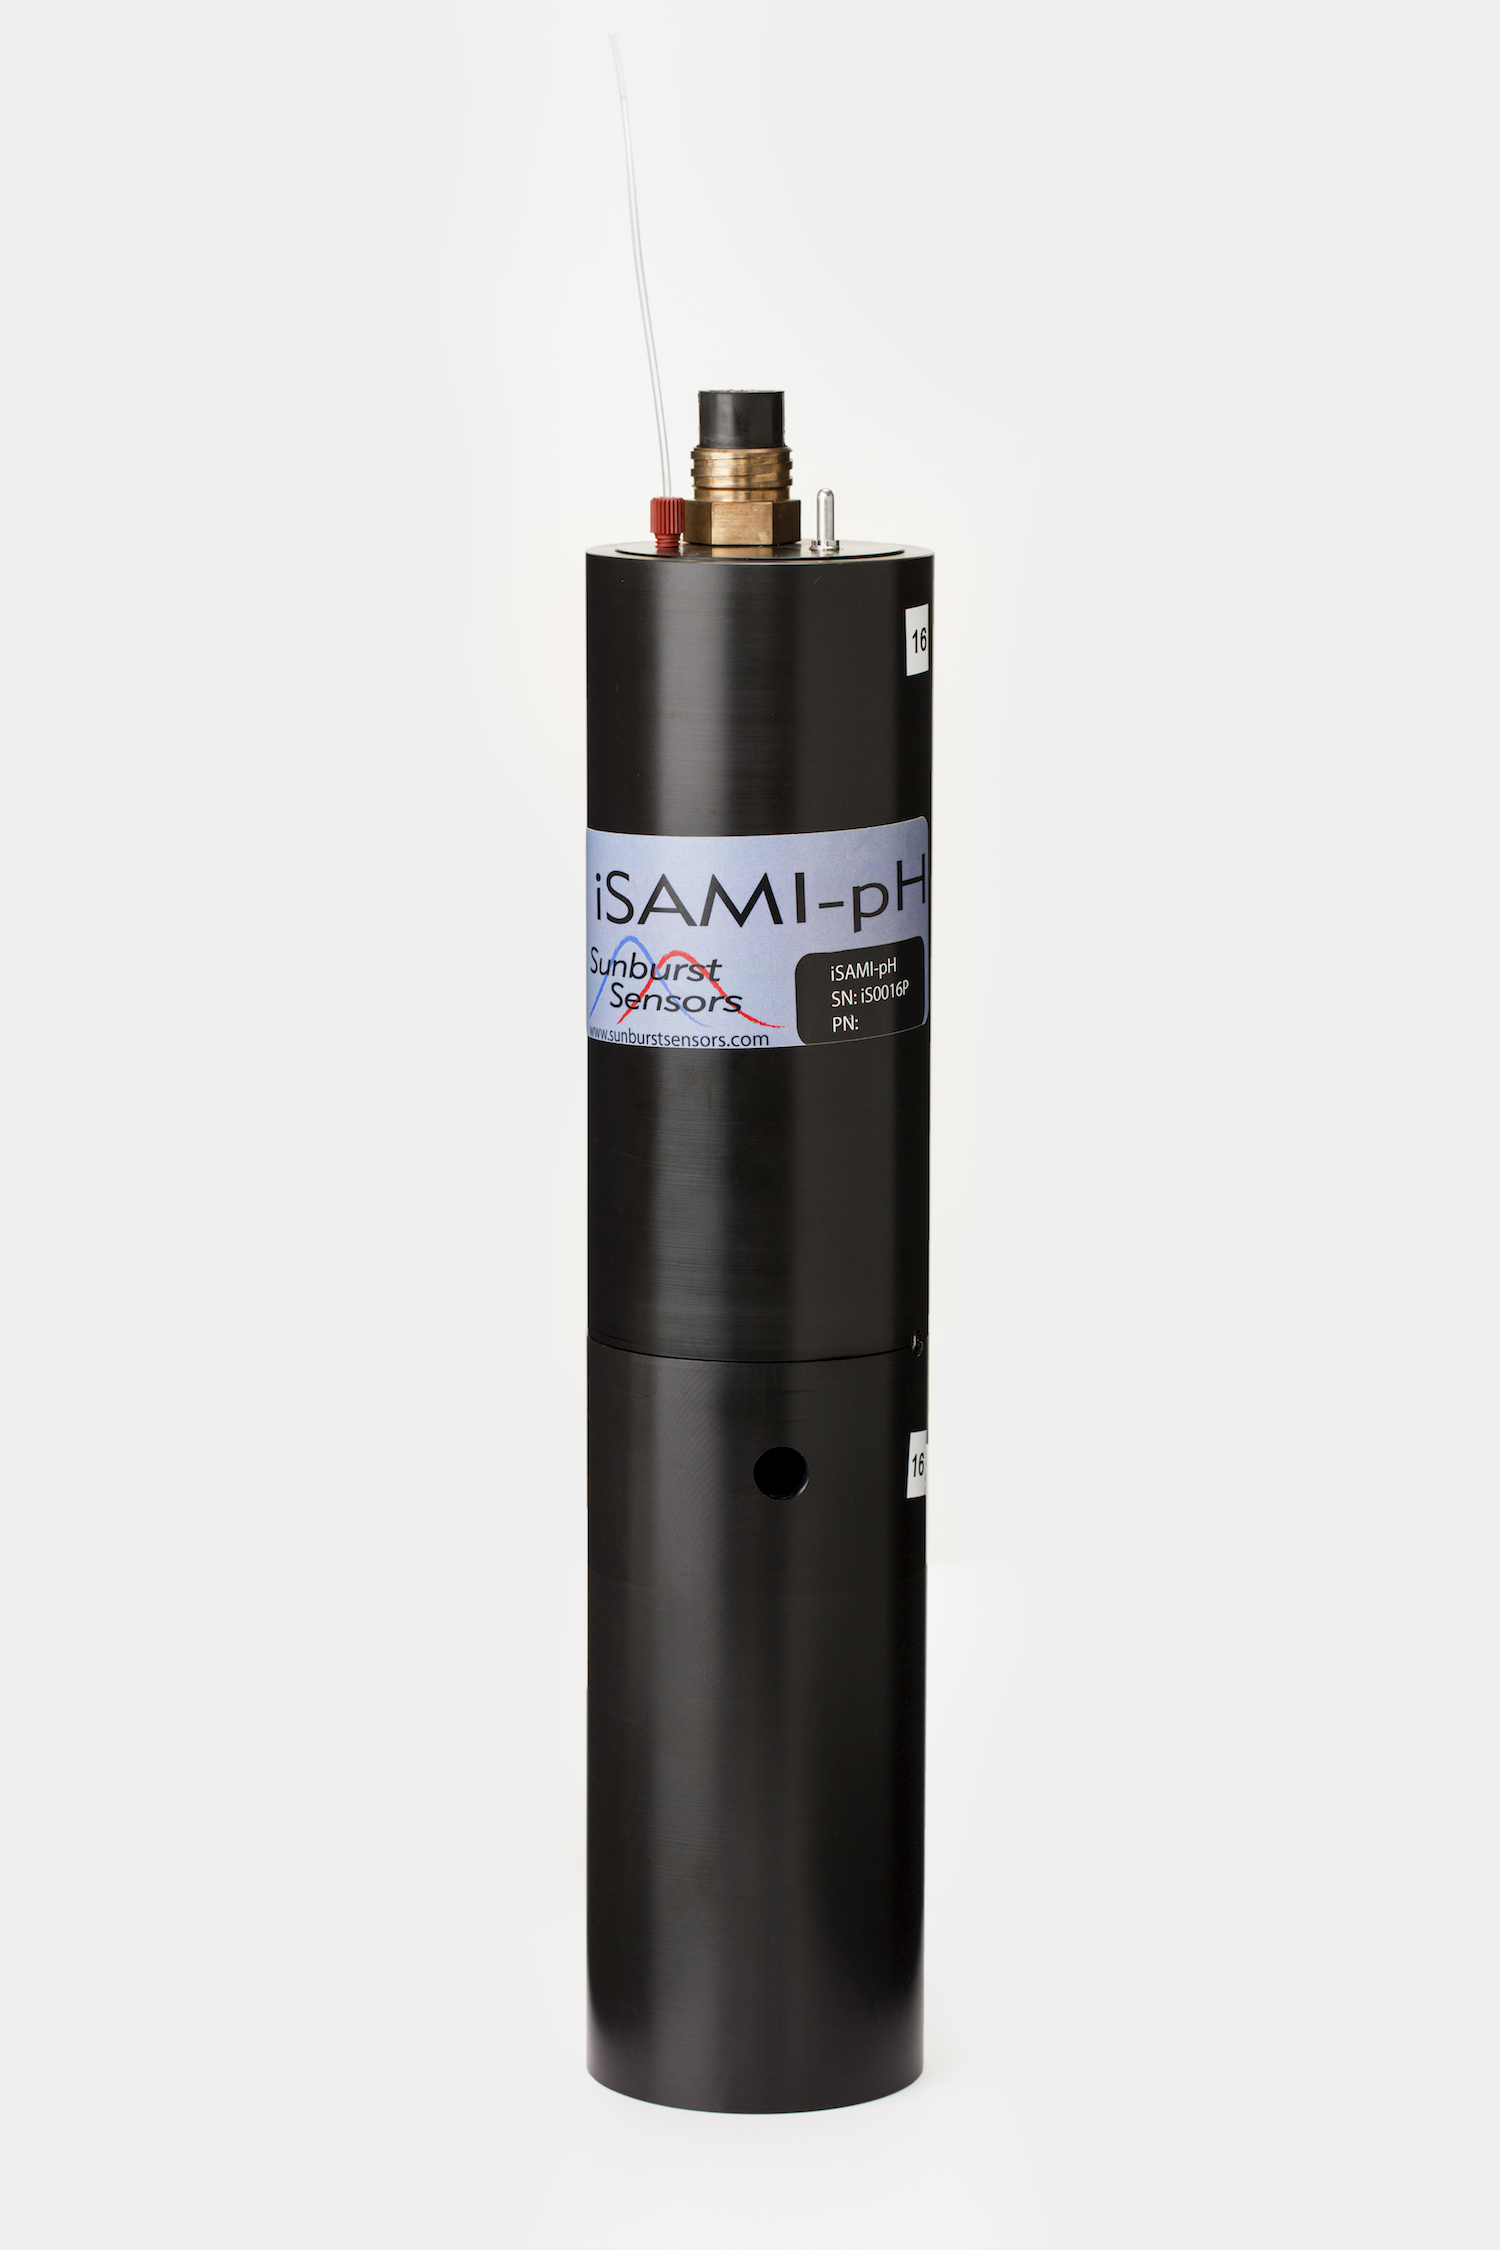
\includegraphics[scale=0.7]{figs/iSAMIsmall.png}
			\end{center}
			\vspace*{\fill}

        \begingroup
            \centering
			\begin{minipage}[b]{0.5\hsize}
			\raggedright
			
\includegraphics[scale=0.7]{figs/SBlogo.jpg}
			\end{minipage}
			\noindent
			\begin{minipage}[b]{0.5\hsize}
			\raggedleft
			\small
            
			Sunburst Sensors, LLC\\
			1226 W Broadway Ave\\
			Missoula, MT 59802\\
			+1 406 532 3247\\
            \url{www.sunburstsensors.com}\\
            info@sunburstsensors.com\\
			\end{minipage}
        \endgroup
			
		\end{nolinenumbers}
\end{titlepage}
\restoregeometry

% Add blank leaf after title page
\newpage\null\thispagestyle{empty}\newpage
\newpage\null\thispagestyle{empty}\newpage

\addtocontents{toc}
{\protect\thispagestyle{empty}}
\tableofcontents
{\protect\thispagestyle{empty}}
\cleardoublepage
% Add blank leaf after contents
\newpage\null\thispagestyle{empty}\newpage
\newpage\null\thispagestyle{empty}\newpage

\setcounter{page}{1}


%%%%%%%%%%%%%%%
%%  Load chapters here  %%
%%%%%%%%%%%%%%%

\cleardoublepage\thispagestyle{empty}
\section{Cleaning your \instType{} for return to Sunburst Sensors}

\noindent
\begin{minipage}[t]{0.5\textwidth}
\centering
\raisebox{\dimexpr \topskip-\height}
{
   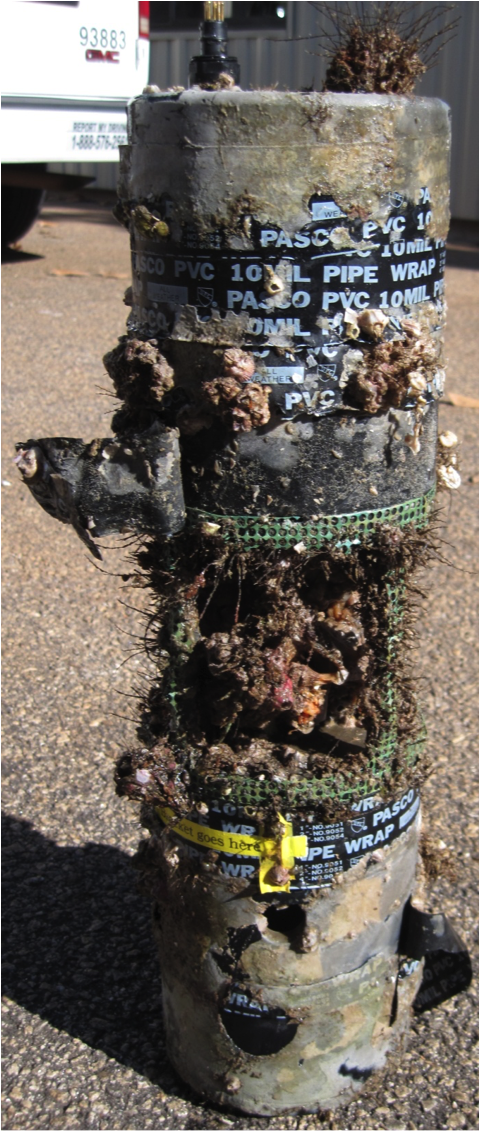
\includegraphics[width=0.9\textwidth]{figs/Foul.png}
}
\end{minipage}
\begin{minipage}[t]{0.5\textwidth}
Please help us speed up your service by properly cleaning your \instType{} before return.  \instType{}s that are returned with excessive biofouling may be subject to additional cleaning and processing charges.\\

\begin{enumerate}
\item Gently remove biological material from the surface of the \instType{}.  Do not use abrasive pads or metal scrapers as these may damage the housing.\\

%\ifiSAMI
%	% If iSAMI don't talk about brass cage and fibers.
%\else
%	\item If there is significant fouling inside the brass cage areas of the instrument, remove the cage and spray a moderate stream of water to remove what will easily come off.  Be careful of the fiber optics and tubing.  The brass cage can be discarded.\\
%\fi

\ifcase \inst
	% If iSAMI don't talk about brass cage and fibers.
\or
	\item If there is significant fouling inside the brass cage areas of the instrument, remove the cage and spray a moderate stream of water to remove what will easily come off.  Be careful of the fiber optics and tubing.  The brass cage can be discarded.\\
\or
	This is an AFT.
\fi

\item After completing the above steps, please allow 24 to 48 hours in a dry area before packing up the instrument. \textbf{Never wrap a wet \instType{} in plastic and return to Sunburst}.
\end{enumerate}

\ifiSAMI
    \vspace*{6.5cm}
\else
    \vspace*{4cm}
\fi

\noindent
To make cleaning easier, 10\,mil PVC corrosion protection tape can be applied to the \instType{} pre-deployment and then removed along with fouling at the end of deployment. This is available from many suppliers such as McMaster Carr:
\newline
\url{http://www.mcmaster.com/#7621A11}
\end{minipage}


\newpage
\restoregeometry

\section{Warnings and Safety}

To prevent damage to the Submersible Autonomous Moored Instrument (\instType{}), please carefully read the operating instructions before attempting to use your instrument. The cable provided is for bench-top programming and download of the \instType{} data, and can be used for shallow laboratory submersion.  IT IS NOT MEANT TO BE DEPLOYED!


\subsection*{Handling}

The \instType{} is reagent-based with the reagent stored in sealed foil bags underneath the instrument.  It is possible, though very unlikely, that these bags may leak or rupture. In case of exposure to the reagent, please refer to the material safety data sheets in the appendix of this manual.


\subsection*{\instType{} Power}

The \instType{} can be powered externally (10--13\,VDC). Observe common safety protocols when using any external power supplies, especially in a wet environment.  While the instrument is diode protected for reverse voltage, large voltages will damage the instrument.  Connect with care!


\section{Introduction to the \instType{}-pH}

\subsection{What's in the box...}

The rugged instrument case for your \instType{} should contain the following upon arrival:

% Use a different list for iSAMI/SAMI
\ifiSAMI
    \begin{enumerate}
    \item \instType{}-pH Instrument.
    \item \instType{} Operating Manual.
    \item Communication/Power Cable.
    \item \instType{} Software Disc.
    \item De-Clogging kit (for air-locked pump).
    \item Pre-Deployment Checklist.
    \item Battery pack (if ordered).
    \end{enumerate}
\else
    \begin{enumerate}
    \item \instType{}-pH Instrument.
    \item \instType{} Operating Manual.
    \item Communication/Power Cable.
    \item \instType{} Software Disc.
    \item De-Clogging kit (for air-locked pump).
    \item Pre-Deployment Checklist.
    \item Any external instruments, extra batteries or reagent ordered, though these may ship separately.
    \item Pre-wetted inlet filter.
    \end{enumerate}
    
    \noindent
    Your stainless steel mooring cage, if ordered for a \instType{}, will ship separately.
\fi

\noindent
If any of these materials is damaged or missing, please contact Sunburst Sensors immediately.


\subsection{Overview of Communication}

\begin{figure}[ht]
\centering
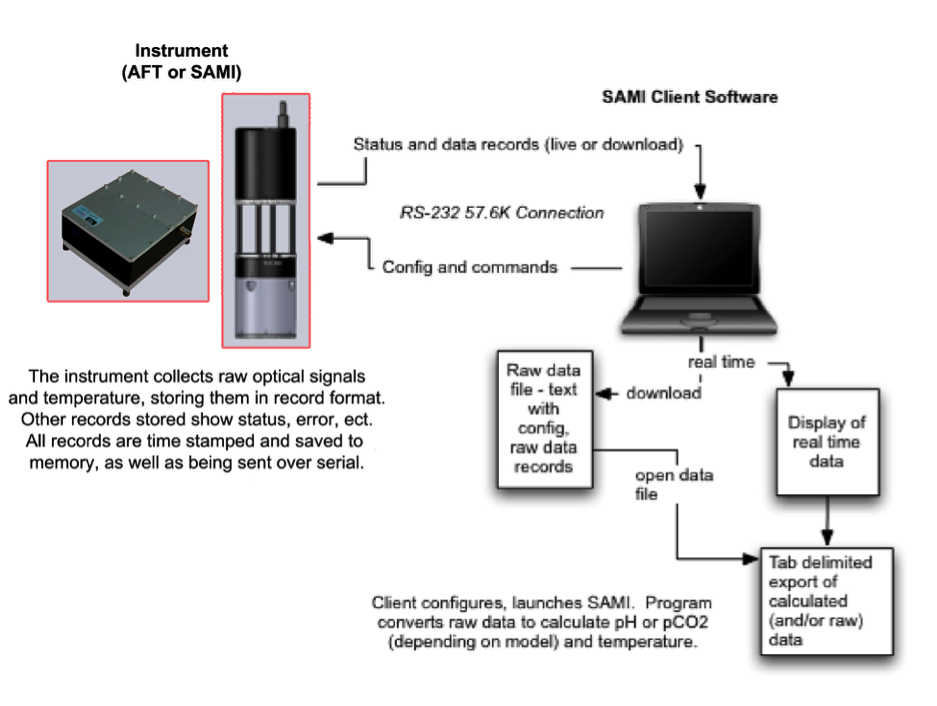
\includegraphics[width=1.0\textwidth]{figs/OperationFig.png}
\caption{Operation overview.}
\label{fig:OperationFig}
\end{figure}

Figure \ref{fig:OperationFig} gives an overview of how the \instType{}-pH operates and interacts with the \textbf{SAMI_Client} software.  The \instType{} uses a time-stamped, records based system to store and transmit data.  There are two main types of records; Data and Status.  Data records consist of raw measurement data, while status records contain information about the state of the instrument (start, stop, battery low, error, etc.)

Once running, all records are stored to internal memory for later download.  Additionally they are transmitted over the serial port, though for energy efficiency the port only wakes up long enough to send the data. 

Data records transmitted to the client can be displayed in real time.

The \textbf{SAMI_Client} software sends configuration data (start time, sampling interval, etc.) and commands to the \instType{} (start, stop, erase, etc.)  It also allows the download of data from the instrument.  Data is downloaded into a text file that contains the configuration data and raw signal intensities as well as any status records.  The user can then open and parse that file using the \textbf{SAMI_Client}.

Data can be exported to tab-delimited files for use in other graphing or analytical software from the data viewer.


\subsection{\instType{}-pH Hardware}

% if SAMI, talk about pressure housing and p/v housing, etc.
\ifiSAMI
    The \instType{} consists of the water sealed electronics housing and the reagent housing.  These are described below.
\else
    The \instType{} consists of a pressure housing, reagent housing, pump/valve housing and the sampling area.  These are described below.
\fi

\ifiSAMI
    \begin{wrapfigure}[25]{r}{0.5\textwidth}
    \centering
       \includegraphics[width=0.9\textwidth]{figs/\instType_pic.png}
    \caption{\instType{}-pH.}
    \label{fig:\instType{}pH}
    \end{wrapfigure}
\else
    \begin{wrapfigure}[32]{r}{0.5\textwidth}
    \centering
       \includegraphics[width=0.9\textwidth]{figs/\instType_pic.png}
    \caption{\instType{}2-pH.}
    \label{fig:\instType{}pH}
    \end{wrapfigure}
\fi


% Use a different list to describe iSAMI/SAMI
\ifiSAMI
    \textbf{Electronics Housing:} The electronics housing contains the controller board, back-up batteries, optics, integrated pump, valve, mixer, and optical cell. \textbf{The \instType{} pump is not pressure-compensated. The \instType{} can therefore only be used from the surface to 3 m depth.} The communication-power bulkhead fitting is located on the top of the housing. The tubing protruding from the top of the \instType{} is the sample outlet.\\
    
    \textbf{Reagent Housing:} The reagent housing, found on the bottom of the instrument, holds and protects the reagent bag but is open to the environment to maintain pressure equilibrium. A bag containing nanopure water or \say{blank} will be attached to the inlet tubing protruding from the reagent housing. This tubing is the sample inlet, and the bag must therefore be removed before deploying the \instType{}. Be careful to not introduce air bubbles when removing the bag.\\
    
    \textbf{Cable:} See Section \ref{Cable}.
\else
    \textbf{Pressure Housing:} The pressure housing contains the controller board, batteries and optics. The communication-power bulkhead fitting is located on the top of the housing. Other bulkhead fittings will be present if external instruments are being supported.\\
    
    \textbf{Sampling Area:} Wrapped in a protective perforated brass housing (not shown), this area is open to the environment. It contains the flow cell, the mixing coil, fiber optics and thermistor. A bag containing nanopure water or \say{blank} will be attached to the inlet tubing protruding from the brass housing. This tubing is the sample inlet, and the bag must therefore be removed before deploying the \instType{}. Be careful to not introduce air bubbles when removing the bag.\\
    
    \textbf{Pump/Valve Housing:} This pressure compensated housing is filled with low viscosity silicon oil to maintain a hydrostatic pressure environment for the pump and valve contained within. A diaphragm on the bottom of the housing makes contact with external pressure. The pump drives reagent through the system, while the valve selects between reagent and seawater.\\
    
    \textbf{Reagent Housing:} The reagent housing, found on the bottom of the instrument, holds and protects the reagent bag but is open to the environment to maintain pressure equilibrium.\\
    
    \textbf{Cable:} See Section \ref{Cable}.
\fi
\cleardoublepage\thispagestyle{empty}
\section{\instType{} Deployment Considerations}

\ifcase \inst	%iSAMI

    The \instType{}-pH is recommended for use in waters with salinity and pH ranges of 25--40 and 7--9, respectively, at temperatures ranging from 0 to 35\,$\degree$C, and depth to 3\,m.

\or			%SAMI

    The \instType{}-pH is recommended for use in waters with salinity and pH ranges of 25-40 and 7-9, respectively, at temperatures ranging from 0 to 35$\degree$C, and depth to 600\,m.  The \instType{} can be configured to measure waters with lower salinity and pH. High pressure rated versions are also available for deeper deployments.  The \instType{}-pH can support and log data for up to three external instruments, such as PAR, dissolved oxygen, CTD, and chlorophyll fluorometer.  Please contact sales or technical support to discuss these options.

\or			%AFT

The \instType{} is intended for measurements of flow-through seawater from a ship sampling line.  Set up is described in Chapter.  Care must be taken to avoid excessive positive or negative pressure in the \instType{} wet chamber.  Excessive pressure can cause seawater to leak into the electronic chamber, destroying optics and electronics.  Negative pressure can cause air bubbles to form in the optical cell, resulting in poor pH precision. 

The \instType{} is a spectrophotometric instrument which discharges a small amount of dye into the seawater stream.  Any instrument located upstream of the \instType{} in the seawater line should not alter the visible spectrum of the seawater.  Instruments located downstream of the \instType{} should not be affected by the dye.  

pH is reported at the temperature in the wet chamber of the \instType{}.  In order to report pH at in situ temperature, in situ temperature must be measured, and the pH should be corrected using the following equation:

\begin{equation}
pH_{is} = {pH_m} + 0.015 ( T_m - T_{is} )
\end{equation}

where $pH_{is}$ is in situ pH, $pH_m$ is pH measured by the \instType{}, $T_{is}$ is in situ temperature in C, and $T_m$ is measured temperature in C.

\fi


\subsection{pH Range}

The measurable pH range of the \instType{}-pH is dictated by the \pKa{} of the indicator, \textit{meta}-cresol purple (\mCP{}), and is 7--9 in the standard configuration.  Below and above this range, absorbances become unreliable, and accuracy degrades.  Different pH indicators in combination with different optics can be used to target a different pH, but the targeted range will not exceed 2 pH units.  Targeting a pH range other than 7--9 requires using an indicator that is not as well characterized as \mCP{}, and could result in less accurate pH measurement.  Table \ref{pH Measurement Range} summarizes available indicators and their pH ranges at salinity of 35. 

\begin{table}[ht]
   \begin{center}
   \caption{\label{pH Measurement Range}pH Measurement Range\\ $^\ast$at salinity 35 and 15$\degree$C}
   \vspace{3mm}
   \centering
   \begin{tabular}{m{30mm} m{30mm} @{}m{0mm}}
      \toprule
      \centering \textbf{Indicator} & \centering \textbf{pH Range$^\ast$} & \\
      \midrule
      \centering thymol blue & \centering 7.5--9.5 & \\
      \midrule
      \centering \textit{meta}-cresol purple & \centering 7.1--9.1 & \\
      \midrule
      \centering phenol red & \centering 6.5--8.5 & \\   
      \midrule
      \centering bromo-cresol purple & \centering 4.9--6.9 &\\
      \bottomrule
   \end{tabular}
   \end{center}
\end{table}


\subsection{Salinity Range}

The \pKa{} of the indicator is dependent on temperature and salinity, and thus both need to be measured for accurate pH measurement.  If salinity is known to $\pm$\,1\,PSU, using the average, constant salinity to calculate the measured pH is adequate.  If salinity varies at the deployment site, salinity should be measured with an external instrument.  \ifcase \inst {} \or {The salinity logged by a \instType{} that is controlling a CTD can be used with \instType{} Client software to calculate pH. If the CTD } \or {The salinity logged by a \instType{} that is controlling a TSG can be used with \instType{} Client software to calculate pH. If the TSG } \fi logs salinity independently, a standalone Matlab routine can be used to calculate pH with the measured salinity.  

\ifcase \inst	%iSAMI

    \instType{}-pH instruments will be accurate to $\pm$\,0.007\,pH through the salinity range of 25--40.  Limited results from lower salinities have given accuracies better than $\pm$\,0.015\,pH.

\else			%SAMI/AFT

    \instType{}-pH instruments will be accurate to $\pm$\,0.004\,pH through the salinity range of 25--40.  Limited results from lower salinities have given accuracies better than $\pm\,$0.015\,pH.
    
\fi

\ifcase \inst	%iSAMI

\or			%SAMI

\or			%AFT

\subsection{Using the \instType{} to measure the pH of discrete samples}

The \instType{}-pH can be configured by Sunburst Sensors to measure the pH of discrete samples. If you intend to use your \instType{} to measure discrete samples, please contact sales or technical support.  In this configuration, the \instType{} will have an additional 3-way solenoid valve to switch between sampling through the wet chamber and sampling through the tubing that comes out the side of the instrument.  When sampling from the tubing, the sample should be placed in a thermostatted water bath. The water bath should be circulated through the wet chamber of the \instType{}, with care to not apply excessive positive or negative pressure.  The inlet tubing should be placed inside the sample.  Failure to circulate thermostatted water through the wet chamber will result in poor accuracy and precision in the pH measurement, as pH is highly temperature sensitive. Note that when measuring the pH of discrete samples, on the \textbf{Settings} tab,
SAMI/AFT panel, bottle must be chosen by entering a 1 in the box.

\fi


\subsection{Measurement Frequency}

\ifcase \inst	%iSAMI

    \begin{table}[ht]
       \begin{center}
       \caption{\label{Reagent Life}Reagent Life}
       \vspace{3mm}
       \centering
       \begin{tabular}{m{30mm} m{30mm} m{30mm}@{}m{0mm}@{}}
          \toprule
          \centering Measurement\newline interval (min) & \centering Measurement\newline frequency ($\mathrm{d^{-1}}$) & \centering \instType{} total reagent life (d), 200\,mL & \\
          \midrule
          \centering 15 & \centering 96 & \centering 83 & \\
          \midrule
          \centering 30 & \centering 48 & \centering 167 & \\   
          \midrule
          \centering 60 & \centering 24 & \centering 333 &\\
          \midrule
          \centering 120 & \centering 12 & \centering 667 & \\ 
          \bottomrule
       \end{tabular}
       \end{center}
    \end{table}

\else			%SAMI/AFT

   \begin{table}[ht]
       \begin{center}
       \caption{\label{Reagent Life}Reagent Life}
       \vspace{3mm}
       \centering
       \begin{tabular}{m{30mm} m{30mm} m{30mm}@{}m{0mm}@{}}
          \toprule
          \centering Measurement\newline interval (min) & \centering Measurement\newline frequency ($\mathrm{d^{-1}}$) & \centering \instType{} total reagent life (d), 550\,mL & \\
          \midrule
          \centering 15 & \centering 96 & \centering 114 & \\
          \midrule
          \centering 30 & \centering 48 & \centering 229 & \\   
          \midrule
          \centering 60 & \centering 24 & \centering 458 &\\
          \midrule
          \centering 120 & \centering 12 & \centering 916 & \\ 
          \bottomrule
       \end{tabular}
       \end{center}
    \end{table}
\fi

\ifcase \inst	%iSAMI

    \begin{table}[ht]
       \begin{center}
       \caption{\label{Battery Life}Battery Life}
       \vspace{3mm}
       \centering
       \begin{tabular}{m{30mm} m{30mm} m{30mm} @{}m{0mm}@{}}
          \toprule
          \centering Measurement\newline interval (min) & \centering Measurement\newline frequency ($\mathrm{d^{-1}}$) & \centering \instType{} total battery life* (d), 0\,$\degree$C & \\
          \midrule
          \centering 15 & \centering 96 & \centering 87 & \\
          \midrule
          \centering 30 & \centering 48 & \centering 174 & \\
          \midrule
          \centering 60 & \centering 24 & \centering 349 & \\
          \midrule
          \centering 120 & \centering 12 & \centering 697& \\
          \bottomrule
       \end{tabular}
       \end{center}
    \end{table}

\else			%SAMI/AFT

    \begin{table}[ht]
       \begin{center}
       \caption{\label{Battery Life}Battery Life}
       \vspace{3mm}
       \centering
       \begin{tabular}{m{30mm} m{30mm} m{30mm} @{}m{0mm}@{}}
          \toprule
          \centering Measurement\newline interval (min) & \centering Measurement\newline frequency ($\mathrm{d^{-1}}$) & \centering \instType{} total battery life* (d), 0\,$\degree$C & \\
          \midrule
          \centering 15 & \centering 96 & \centering 58 & \\
          \midrule
          \centering 30 & \centering 48 & \centering 117 & \\
          \midrule
          \centering 60 & \centering 24 & \centering 234 & \\
          \midrule
          \centering 120 & \centering 12 & \centering 468 & \\
          \bottomrule
       \end{tabular}
       \end{center}
    \end{table}
    
\fi

By collecting a higher quantity of data points you will more quickly use reagent, battery life, and memory, which will shorten the longevity of your collection time. We encourage you to weigh your options to maximize the effectiveness of your deployment while considering the questions you are trying to answer through your research. Use the tables included above to help you decide upon the appropriate parameters for your deployment.


\ifcase \inst	%iSAMI

\subsection{Cold Water Deployment}

The \instType{}-pH indicator contains NaCl equal to salinity 35, which will prevent the indicator from freezing in seawater.  However, water or indicator inside the narrow gauge tubing will freeze quickly if the \instType{} is kept at below-freezing temperatures for very long.  This will result in loss of data until ice within the tubing melts.  If you are planning to deploy your \instType{}-pH in below-freezing weather, we recommend that you take the following precautions to avoid data loss:

\begin{enumerate}
\item
Remove the copper bell attached to the sample inlet \ifcase \inst {tube.} \or {tube (this tube extrudes from and is zip-tied to the brass cage).} \fi Ice can form around the copper bell if it has water in it.
\item
Please let the sales or technical staff at Sunburst know about the cold weather deployment, and request a blank bag with 10\,\% ethylene glycol. Ethylene glycol will decrease the freezing temperature of the water in the bag.
\item
Minimize the amount of time that your \instType{}-pH is exposed to cold weather before deploying.
\end{enumerate}

\or			%SAMI

\subsection{Cold Water Deployment}

The \instType{}-pH indicator contains NaCl equal to salinity 35, which will prevent the indicator from freezing in seawater.  However, water or indicator inside the narrow gauge tubing will freeze quickly if the \instType{} is kept at below-freezing temperatures for very long.  This will result in loss of data until ice within the tubing melts.  If you are planning to deploy your \instType{}-pH in below-freezing weather, we recommend that you take the following precautions to avoid data loss:

\begin{enumerate}
\item
Remove the copper bell attached to the sample inlet \ifcase \inst {tube.} \or {tube (this tube extrudes from and is zip-tied to the brass cage).} \fi Ice can form around the copper bell if it has water in it.
\item
Please let the sales or technical staff at Sunburst know about the cold weather deployment, and request a blank bag with 10\,\% ethylene glycol. Ethylene glycol will decrease the freezing temperature of the water in the bag.
\item
Minimize the amount of time that your \instType{}-pH is exposed to cold weather before deploying.
\end{enumerate}

\or			%AFT

\fi


\ifcase \inst	%iSAMI

\subsection{Deployment in High TDS or Highly Productive Areas}

The \instType{}-pH pumps about 3\,mL of seawater through the system for every pH measurement.  The hardware can become clogged or malfunctional and optical throughput can degrade due to fine particles or biological fouling.  An inlet filter was shipped with your \instType{}-pH.  Use the following guide to decide whether to use it.

\textbf{Use the inlet filter} if you will be deploying in a high fouling or silty area.  Be advised that this might cause some degree of resolution loss if the pH is highly variable.  You can increase the number of flush pumps if necessary, although this will decrease battery life.  We believe that it might be necessary to change the filter during deployment if it becomes highly fouled, but we cannot give advice as to how long the filter will work for.  Order extra filters if you think you will need them.

\textbf{Use the copper bell} if you are not concerned about fouling due to deep, cold, or non-productive water.  You can also deploy with the copper bell (without the filter) if you want to be sure to completely resolve pH when it is rapidly changing,  Be advised that the \instType{} might foul after a month or two and begin to give erratic data if the water is highly productive.

\textbf{Remove the copper bell} if you are deploying in cold temperatures and are concerned about the \instType{} fluids freezing during the time that the \instType{} is exposed to freezing temperatures prior to deployment.

Refer to Figure \ref{fig:FilterFig}  when following instructions for \instType{} inlet configuration.


\subsubsection{Instructions for inlet filter use}

\begin{enumerate}
\item
Unscrew the white union inside the copper bell (A).
\item
Approximately 1 inch of tubing will protrude from the blue nut (B).  The copper bell can be left on or removed.
\item 
The filter is pre-wetted with isopropyl alcohol.  It is shipped with a small amount of deionized water to deep it wet, but there may be a residual amount of alcohol in the bag (C).
\item
Insert the tubing into the filter and connect using the blue nut.  The tubing will go all the way to the bottom of the filter (D).
\item
Remove the blank bag by cutting the zip tie.  A plug for the bag is included with the flushing syringe (E).
\item
Secure the filter with a zip tie before deployment (E).
\end{enumerate}


\subsubsection{Instructions for copper bell use}

\begin{enumerate}
\item
Unscrew the white union inside the copper bell (A).
\item
Approximately 1 inch of tubing will protrude from the blue nut (B).
\item
Using a razor or other sharp edge, cut the tubing flush with the blue nut, being careful to not crimp the tubing end (F).
\item
Remove the blank bag by cutting the zip tie (E).  A plug for the bag is included with the flushing syringe.
\end{enumerate}


\subsubsection{Instructions for bare tubing use}

\begin{enumerate}
\item
Unscrew the white union inside the copper bell (A).
\item
Approximately 1 inch of tubing will protrude from the blue nut (B).
\item
Unscrew the copper bell (G).
\item
Using a razor or other sharp edge, cut the tubing flush with the blue nut, being careful to not crimp the tubing end (G).
\item
Remove the blank bag by cutting the zip tie (E).  A plug for the bag is included with the flushing syringe.
\end{enumerate}

\begin{figure}
\centering
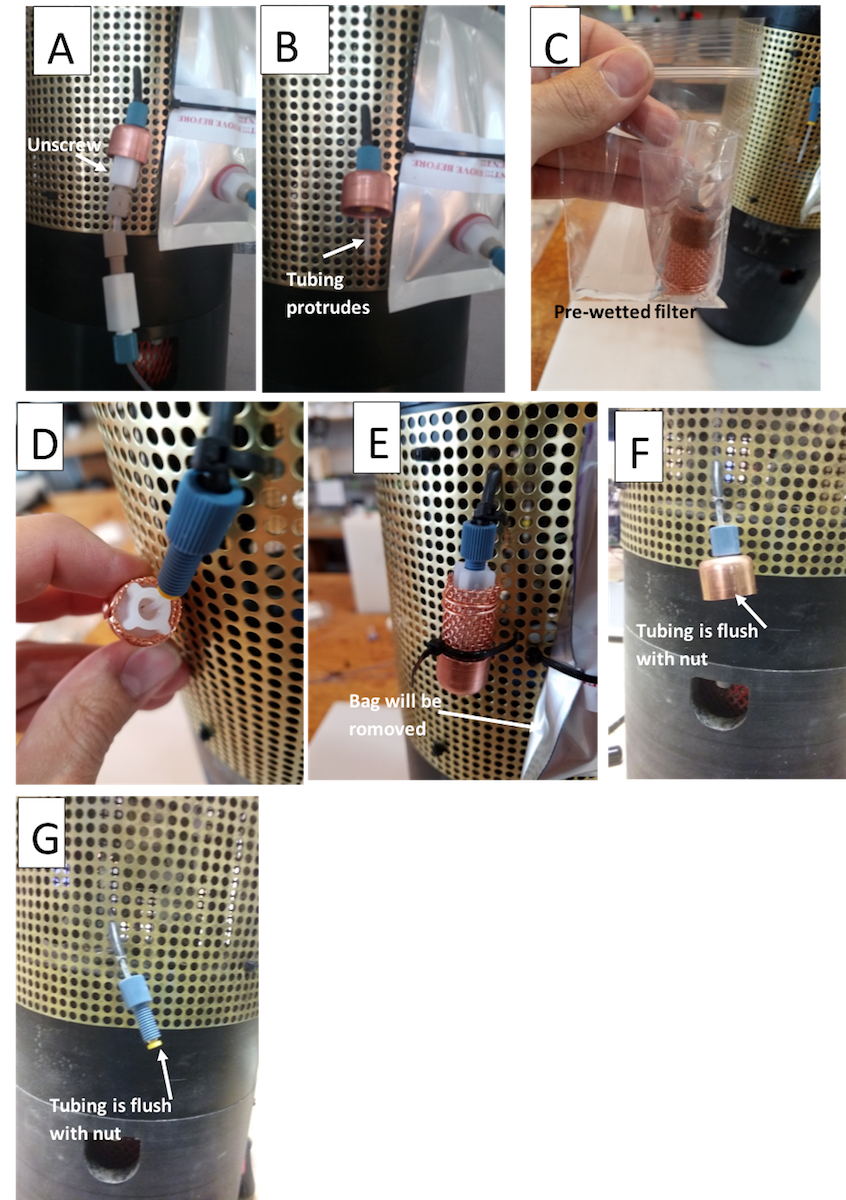
\includegraphics[width=1.0\textwidth]{figs/Filter_Fig.png}
\caption{\instType{} inlet configuration}
\label{fig:FilterFig}
\end{figure}

\or		%SAMI

\subsection{Deployment in High TDS or Highly Productive Areas}

The \instType{}-pH pumps about 1\,mL of seawater through the system for every pH measurement.  The hardware can become clogged or malfunctional and optical throughput can degrade due to fine particles or biological fouling.  An inlet filter was shipped with your \instType{}-pH.  Use the following guide to decide whether to use it.  If you are concerned about the \instType{} failing due to highly productive or silty water, please contact technical support to request an inlet filter.  This filter will cause loss of resolution and will require more pumping, which will drain the battery faster.

\textbf{Use the inlet filter} if you will be deploying in a high fouling or silty area.  Be advised that this might cause some degree of resolution loss if the pH is highly variable.  You can increase the number of flush pumps if necessary, although this will decrease battery life.  We believe that it might be necessary to change the filter during deployment if it becomes highly fouled, but we cannot give advice as to how long the filter will work for.  Order extra filters if you think you will need them.

\textbf{Use the copper bell} if you are not concerned about fouling due to deep, cold, or non-productive water.  You can also deploy with the copper bell (without the filter) if you want to be sure to completely resolve pH when it is rapidly changing,  Be advised that the \instType{} might foul after a month or two and begin to give erratic data if the water is highly productive.

\textbf{Remove the copper bell} if you are deploying in cold temperatures and are concerned about the \instType{} fluids freezing during the time that the \instType{} is exposed to freezing temperatures prior to deployment.

Refer to Figure \ref{fig:FilterFig}  when following instructions for \instType{} inlet configuration.


\subsubsection{Instructions for inlet filter use}

\begin{enumerate}
\item
Unscrew the white union inside the copper bell (A).
\item
Approximately 1 inch of tubing will protrude from the blue nut (B).  The copper bell can be left on or removed.
\item 
The filter is pre-wetted with isopropyl alcohol.  It is shipped with a small amount of deionized water to deep it wet, but there may be a residual amount of alcohol in the bag (C).
\item
Insert the tubing into the filter and connect using the blue nut.  The tubing will go all the way to the bottom of the filter (D).
\item
Remove the blank bag by cutting the zip tie.  A plug for the bag is included with the flushing syringe (E).
\item
Secure the filter with a zip tie before deployment (E).
\end{enumerate}


\subsubsection{Instructions for copper bell use}

\begin{enumerate}
\item
Unscrew the white union inside the copper bell (A).
\item
Approximately 1 inch of tubing will protrude from the blue nut (B).
\item
Using a razor or other sharp edge, cut the tubing flush with the blue nut, being careful to not crimp the tubing end (F).
\item
Remove the blank bag by cutting the zip tie (E).  A plug for the bag is included with the flushing syringe.
\end{enumerate}


\subsubsection{Instructions for bare tubing use}

\begin{enumerate}
\item
Unscrew the white union inside the copper bell (A).
\item
Approximately 1 inch of tubing will protrude from the blue nut (B).
\item
Unscrew the copper bell (G).
\item
Using a razor or other sharp edge, cut the tubing flush with the blue nut, being careful to not crimp the tubing end (G).
\item
Remove the blank bag by cutting the zip tie (E).  A plug for the bag is included with the flushing syringe.
\end{enumerate}

\begin{figure}
\centering
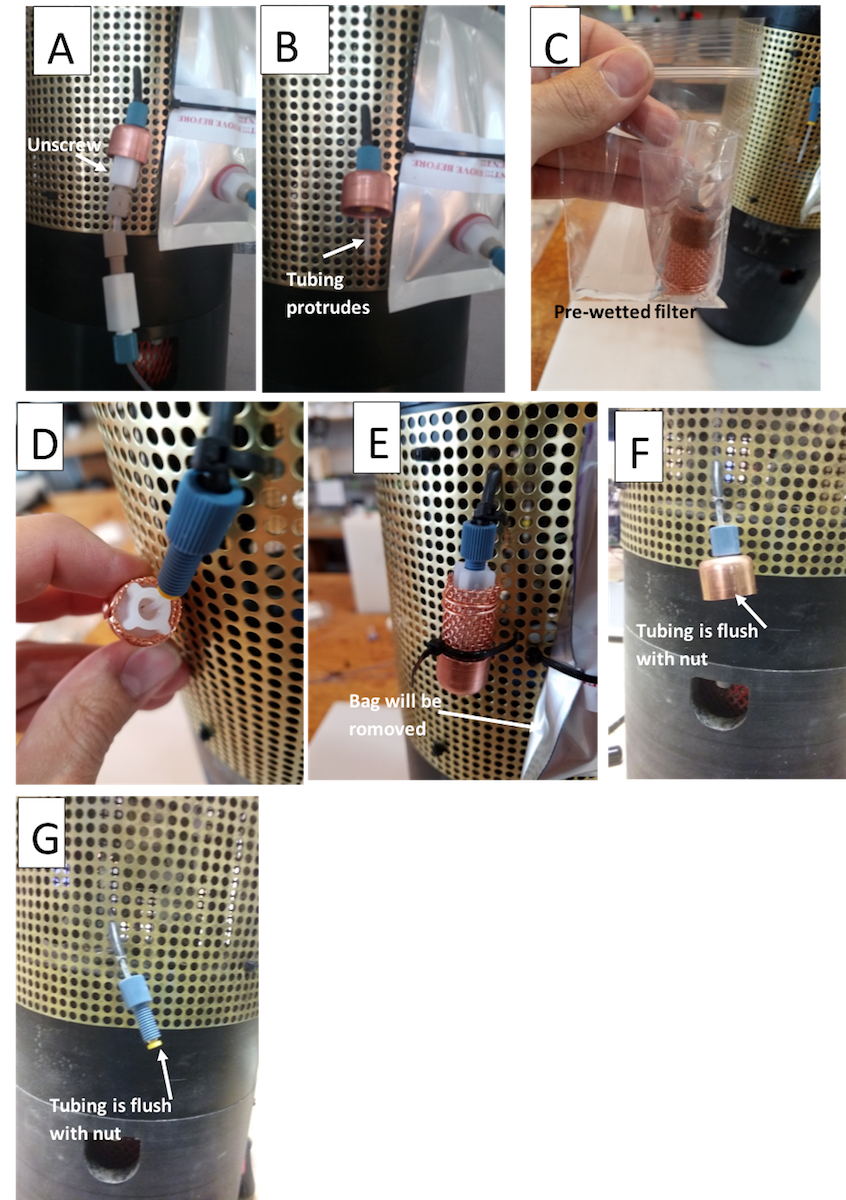
\includegraphics[width=1.0\textwidth]{figs/Filter_Fig.png}
\caption{\instType{} inlet configuration}
\label{fig:FilterFig}
\end{figure}


\subsection{Avoiding Air-Lock}

Care must be taken to avoid deploying the \instType{}-pH with air in the tubing, or pumping the \instType{} when it is not either connected to the blank bag or immersed in water.  If the \instType{} tubing is full of air when it is deployed, this can cause the pumps to lock up, and no useful data will be collected.  

Before deploying the \instType{}-pH, flush with blank.  Leave the blank bag connected to the inlet and perform a pH flush using the \instType{} client software as described in section \ref{sec:AirLock}.  After flushing is complete, set the sample start to a time well after deployment is expected. Be sure to remove the blank bag from the inlet before deploying.

\fi
\cleardoublepage\thispagestyle{empty}
\section{\instType{}-pH Theory of Operation}

\mCP{}, a pH sensitive dye that has been purified to use in \instType{} instruments to increase measurement accuracy (Liu et al 2011).  A seawater sample stream is pumped through the instrument and injected with a pH-sensitive indicator solution (\mCP{}). Two wavelength-specific LEDs send alternating pulses of light through the indicator-sample mixture as it is pumped through a flow cell. Changes in absorbance at the two wavelengths, Beer's law, and the known molar absorptivities of the indicator can be used to calculate the concentration of protonated and un-protonated indicator.  The indicator \pKa is then used to calculate pH using a derivation of the Henderson-Hasselbach equation. 


\subsection{Equilibrium Reaction}

Spectrophotometric pH determination is based on the equilibrium reaction of a pH-dependent indicator. A diprotic sulfonephthalein indicator, \mCP{}, is used as the reagent. \ifcase \inst {A single 25\,$\mathrm{\mu L}$ pulse} \else {A single 50\,$\mathrm{\mu L}$ pulse} \fi of reagent is introduced into the seawater stream. The acidic (\ce{HI-}) and basic (\ce{I$^{2-}$}) forms of the indicator are found in varying quantities based on the pH of the seawater being tested.

Indicator equilibrium is described by Equation \ref{eq:equilibrium}:

\begin{equation}
\label{eq:equilibrium}
\ce{HI- <=>[{K_a}'] H+ + I^2-}
\end{equation}

where ${K_a}'$ is the apparent dissociation constant. The acidic and basic forms of the indicator are measured at peak absorbance wavelengths of 434\,nm (\ce{HI-}) and 578\,nm (\ce{I$^{2-}$}), respectively. The diprotic \ce{H2I} form is not present at seawater pH and therefore is not considered in our applications.

Combining the log form of the indicator equilibrium expression, Beer's Law, and the Henderson-Hasselbalch equations results in Equation \ref{eq:H-H}.

\begin{equation}
\label{eq:H-H}
pH = {pK_a}' + log \left(\frac{R - e_1}{e_2 - R e_3}\right),
\end{equation}

where ${pK_a}'$ is the log of the apparent dissociation constant, $R$ is the absorbance ratio $A_{578}/A_{434}$ and the $e_i$ are the temperature-dependent ratios of the molar absorptivities ($\epsilon$) of \ce{HI-} and \ce{I$^{2-}$} at 434 and 578\,nm. Equations 3--10 define temperature-dependent values for $pK_a$$'$ and $e_i$ used for purified \mCP in \instType{} instruments. $T$ is temperature in Kelvin, $t$ is temperature in Celcius, and $S$ is salinity.

\begin{equation}
\label{eq:pKa}
  \begin{aligned}
 {pK_a}' = &-241.462 + 7085.72T^{-1} + 43.8332ln(T) - 0.0806406T - 0.3238S^{0.5} + 0.0807S\\
           & - 0.01157S^{1.5} + 0.000694S^2 + 0.6367
   \end{aligned}
\end{equation}

\begin{equation}
\label{eq:e1}
e_1 = {\epsilon}a_{578}/{\epsilon}a_{434}
\end{equation}

\begin{equation}
\label{eq:e2}
e_2 = {\epsilon}b_{578}/{\epsilon}a_{434}
\end{equation}

\begin{equation}
\label{eq:e3}
e_3 = {\epsilon}b_{434}/{\epsilon}a_{434}
\end{equation}

\begin{equation}
\label{eq:ea434}
{\epsilon}a_{434} = 17372 + 20.162(24.80 - t)
\end{equation}

\begin{equation}
\label{eq:ea578}
{\epsilon}a_{578} = 94.1 - 1.0177(24.80 - t)
\end{equation}

\begin{equation}
\label{eq:eb434}
{\epsilon}b_{434} = 2284.1 - 6.3863(24.86 - t)
\end{equation}

\begin{equation}
\label{eq:eb578}
{\epsilon}b_{578} = 38676 + 66.808(24.86 - t)
\end{equation}


\subsection{Optical Path}

The \instType{} uses pulsed LEDs with narrow band filters at wavelengths corresponding to maximum optical absorbance for the protonated and deprotonated forms of the reagent.  A reference photodiode tracks changes in the light sources.  LEDs are imbedded in the flow cell which is mounted on the controller board.  The flow-cell optical path length is 1\,cm. 


\subsection{Fluid Path}

The \instType{}-pH uses a \ifcase \inst {25\,$\mathrm{\mu L}$} \else {50\,$\mathrm{\mu L}$} \fi solenoid pump to drive reagent through the system. A solenoid valve allows the same pump to introduce a single pulse of reagent into the stream for each pH measurement. A card with engraved cicuitous flowpath upstream of the flow cell ensures thorough mixing of the sample and reagent prior to optical measurements. The sample's blank signal intensity ($I_0$) is established by taking measurements while pumping pure sample through the flow cell.  After measuring the blank signal, reagent is introduced into the flow stream and signal intensity ($I$) is collected as the pump pushes the mixture through the flow-cell.  At each measurement, reference intensities ($I_{0_{ref}}$ and $I_{ref}$) are also measured.  The absorbance at each wavelength is calculated as:

\begin{equation}
\label{eq:Abs}
A = -log \left( \frac{I}{I_0}\times \frac{I_{0_{ref}}}{I_{ref}} \right)
\end{equation}


\subsection{pH Perturbation and Data Record}

Each pH data record consists of 28 light intensity measurements at each wavelength.  The first four measurements are averaged and used as the blank intensity values ($I_0$).  pH and indicator concentration are calculated for each of the subsequent measurements.  The addition of the \mCP indicator will slightly alter the pH of the sample. The pH of the initial sample is determined by extrapolating to the pH at zero indicator concentration using a regression of pH vs. indicator concentration (Seidel et al. 2008).


\subsection{Validation}

The \instType{}-pH is validated by measuring the pH of Tris buffer at $\sim$\,25\,$\degree$C. pH accuracy is better than or equal to \ifcase \inst {$\pm$\,0.007} \else {$\pm$\,0.004} \fi at the time the \instType{} is sent to the customer.


\subsection{References}

For more information see the following references:

Delvalls, T.A., Dickson, A.G., 1998.  The pH of Buffers Based on 2-amino-2-hydroxymethyl-1,3-propanediol. Deep-Sea Research I, 45, 1541--1554.

Liu, X., Patsavas, M.C., Byrne, R.H., 2011. Purification and Characterization of meta-Cresol Purple for Spectrophotometric Seawater pH Measurements.  Environmental Science and Technology, 45, 4862--4868.

DeGrandpre, M.D., Spaulding, R.S., Newton, J.O., Jaqueth, E.J., Hamblock, S.E., Umansky, A.A., Harris, K.E, 2014. Considerations for the measurement of spectrophotometric pH for ocean acidification and other studies. Limnology and Oceanography: Methods. 12, 830--839.

Martz, T.R., Carr, J.J., French, C.R., DeGrandpre, M.D., 2003. A submersible autonomous sensor for spectrophotometric pH measurements of natural waters. Anal. Chem, 75, 1844--1850

Seidel, M.P., DeGrandpre, M.D., Dickson, A.G., 2008. A sensor for in situ indictor-based measurements of seawater pH. Mar Chem. 109, 18--28.
\cleardoublepage\thispagestyle{empty}
\section{\instType{} Client Software}
\label{sec:Software}

The \instType{}-pH requires the use of its own client software for programming, download and data interpretation.


\subsection{\instType{} Client Installation}
\label{sec:Install}

\instType{} software is available for both Windows (XP and later) and Mac (OS X).  To install the software, simply insert the \instType{} Software disc, navigate to the \textbf{SAMI\_Client Application} folder and drag the folder for your computer platform to an appropriate location on your hard drive.  You may want to create a shortcut to your application, but it is important that the application itself remain in the folder with the various sub-folders and other files for it to operate correctly.  When you open the \instType{} Client, if connected to the internet, the software will automatically search for updates.  You can update your software at \url{http://www.sunburstsensors.com/swupdate}


\subsubsection{USB Serial Driver}

Also on the disc is the driver for the serial-USB converter that is part of your communication cable. Most modern computers will already have appropriate drivers installed or automatically install this driver from the internet.  If your computer does not recognize the USB-serial converter when the cable is plugged in, you can opt to install from this folder.  You may also use the internet to download the latest driver from \url{http://ftdichip.com/Drivers/VCP.htm}


\subsubsection{\instType{} Cables and Bulkheads}
\label{Cable}

\ifcase \inst	%iSAMI

The black communication cable included with your instrument will have a 6-pin bulkhead connector on one end and on the other end, two diverging cables: a USB and banana plugs. 

The black (ground) and red (positive) banana plugs should be connected to a DC power supply set to 10--13\,VDC. The USB connects directly to one of your computer's USB ports.

The \instType{} uses wet-pluggable bulkhead connections made by Impulse or SubConn.  To communicate with the \instType{}, remove the bulkhead cover plug by unscrewing the locking collar and pulling firmly up. Take care to not unscrew the bulkhead itself, which requires adequate torque (15\,in-lb or 1.7\,Nm) to maintain its seal. To connect the communication/power cable, align the pins on the cable with the receptacles on the \instType{} bulkhead and push down firmly.

The \instType{} uses the RS-232 communication protocol. Figure \ref{fig:Subconn} shows the pin-out of the bulkhead as you look down on it.

The Tx line transmits data out and while the Rx line is how commands are sent to the unit. The RTS line tells the \instType{} that it is connected to the client software. While it is held high the \instType{} will send out status strings about once per second. If connecting to a terminal, or external logger, keep RTS off.  RTS on the client software expires after three minutes to save power (See section \ref{sec:Software}).

    \textbf{The \instType{} internal battery has enough power to maintain the datalogger for about 90 days. Once the internal batteries die, your \instType{} will not be able to store data.} Therefore, the recommended sequence for storing, programming, powering, and running, the \instType{} is:
    
    \begin{enumerate}
    \item[]\textbf{\instType{} storage}. When storing the \instType{}, it should be left connected to a 12\,V battery pack or 12\,VDC power, in order to avoid draining the internal battery.
    
    \item[]\textbf{Running the \instType{} in the lab.} When running the \instType{} in the lab, it must be connected to 12\,VDC power.  The \instType{} will shut down if you attempt to run the pumps or a pH measurement using the internal batteries.
    
    \item[]\textbf{Programming the \instType{} for deployment.} The \instType{} can be programmed while connected to a computer, without external power.
    
    \item[]\textbf{Deploying the \instType{}.} The \instType{} must be connected to a 12\,V submersible battery pack or a 12\,VDC power supply during deployment.  The \instType{} will shut down when the 12\,V supply is removed.
    
    \item[]\textbf{Downloading data from the \instType{} after deployment.} Data can be downloaded from the \instType{} by disconnecting the 12\,V power and connecting the \instType{} to a computer.
    \end{enumerate}

\begin{figure}[t]
\centering
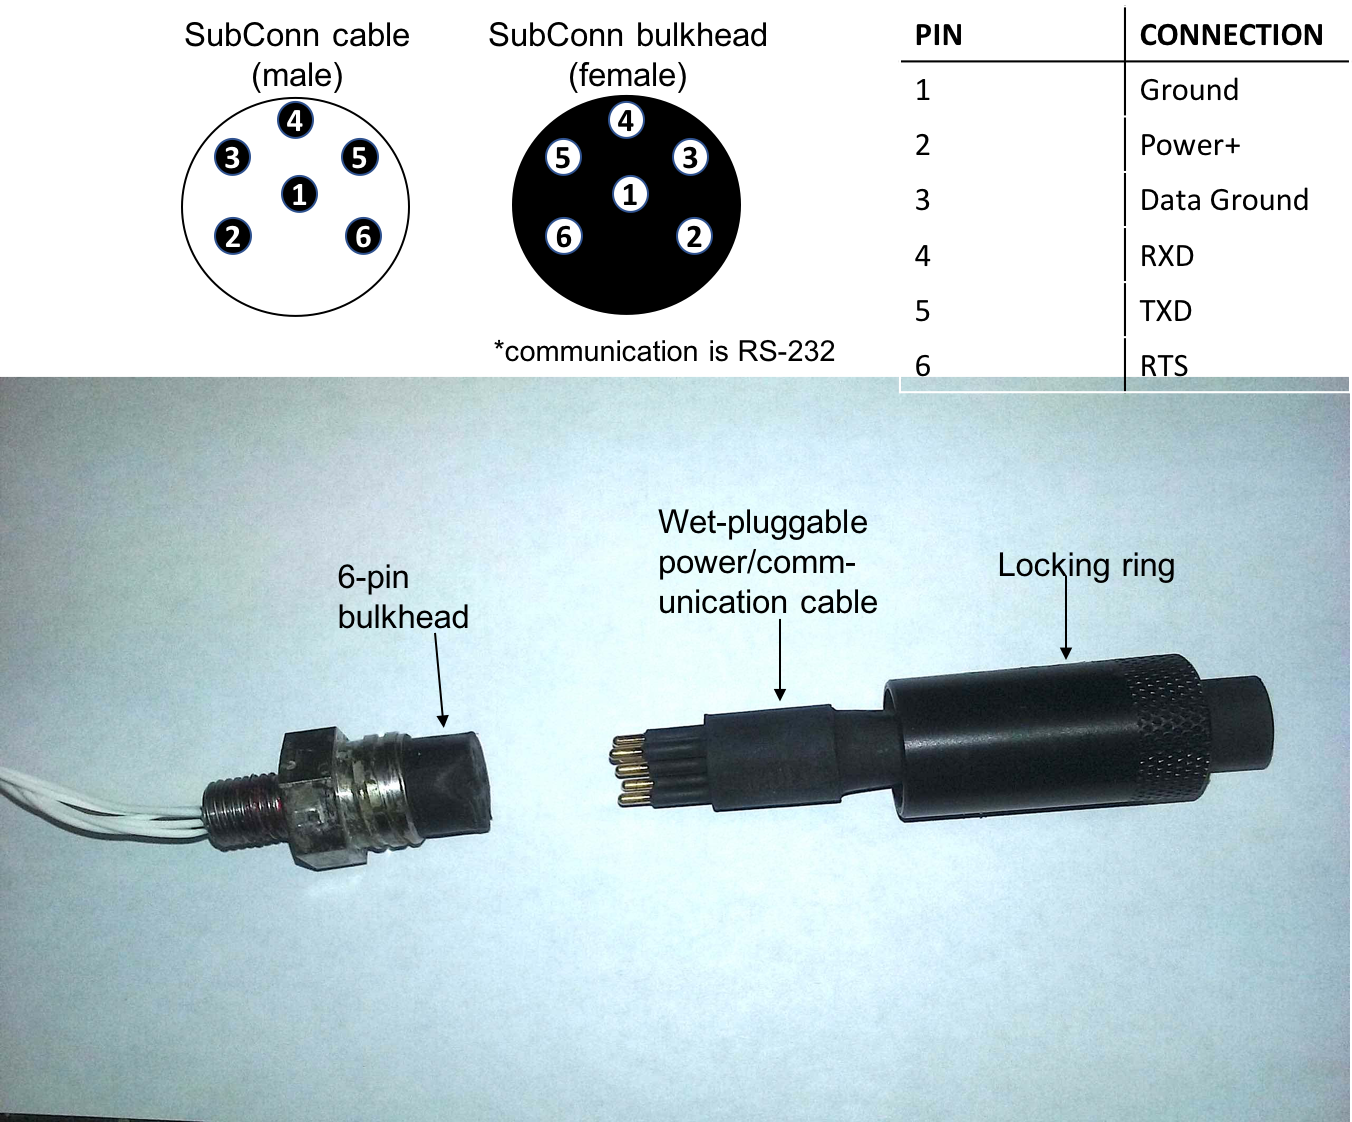
\includegraphics[width=0.8\textwidth]{figs/Subconn_cable.png}
\caption{\instType{} 6-pin connection.}
\label{fig:Subconn}
\end{figure}

\or		%SAMI

The black communication cable included with your instrument will have a 6-pin bulkhead connector on one end and on the other end, two diverging cables: a USB and banana plugs. 

The black (ground) and red (positive) banana plugs should be connected to a DC power supply set to 10--13\,VDC. If the voltage of the power supply is set to be greater than the voltage of the internal batteries, battery power can be saved. The USB connects directly to one of your computer's USB ports.

The \instType{} uses wet-pluggable bulkhead connections made by Impulse or SubConn.  To communicate with the \instType{}, remove the bulkhead cover plug by unscrewing the locking collar and pulling firmly up. Take care to not unscrew the bulkhead itself, which requires adequate torque (15\,in-lb or 1.7\,Nm) to maintain its seal. To connect the communication/power cable, align the pins on the cable with the receptacles on the \instType{} bulkhead and push down firmly. Before deploying the \instType{} be sure to replace the bulkhead cover pug and screw down the locking sleeve to protect the bulkhead pins from corrosion.

The \instType{} uses the RS-232 communication protocol. Figure \ref{fig:Subconn} shows the pin-out of the bulkhead as you look down on it.

The Tx line transmits data out and while the Rx line is how commands are sent to the unit. The RTS line tells the \instType{} that it is connected to the client software. While it is held high the \instType{} will send out status strings about once per second. If connecting to a terminal, or external logger, keep RTS off.  RTS on the client software expires after three minutes to save power (See section \ref{sec:Software}).

\begin{figure}[t]
\centering
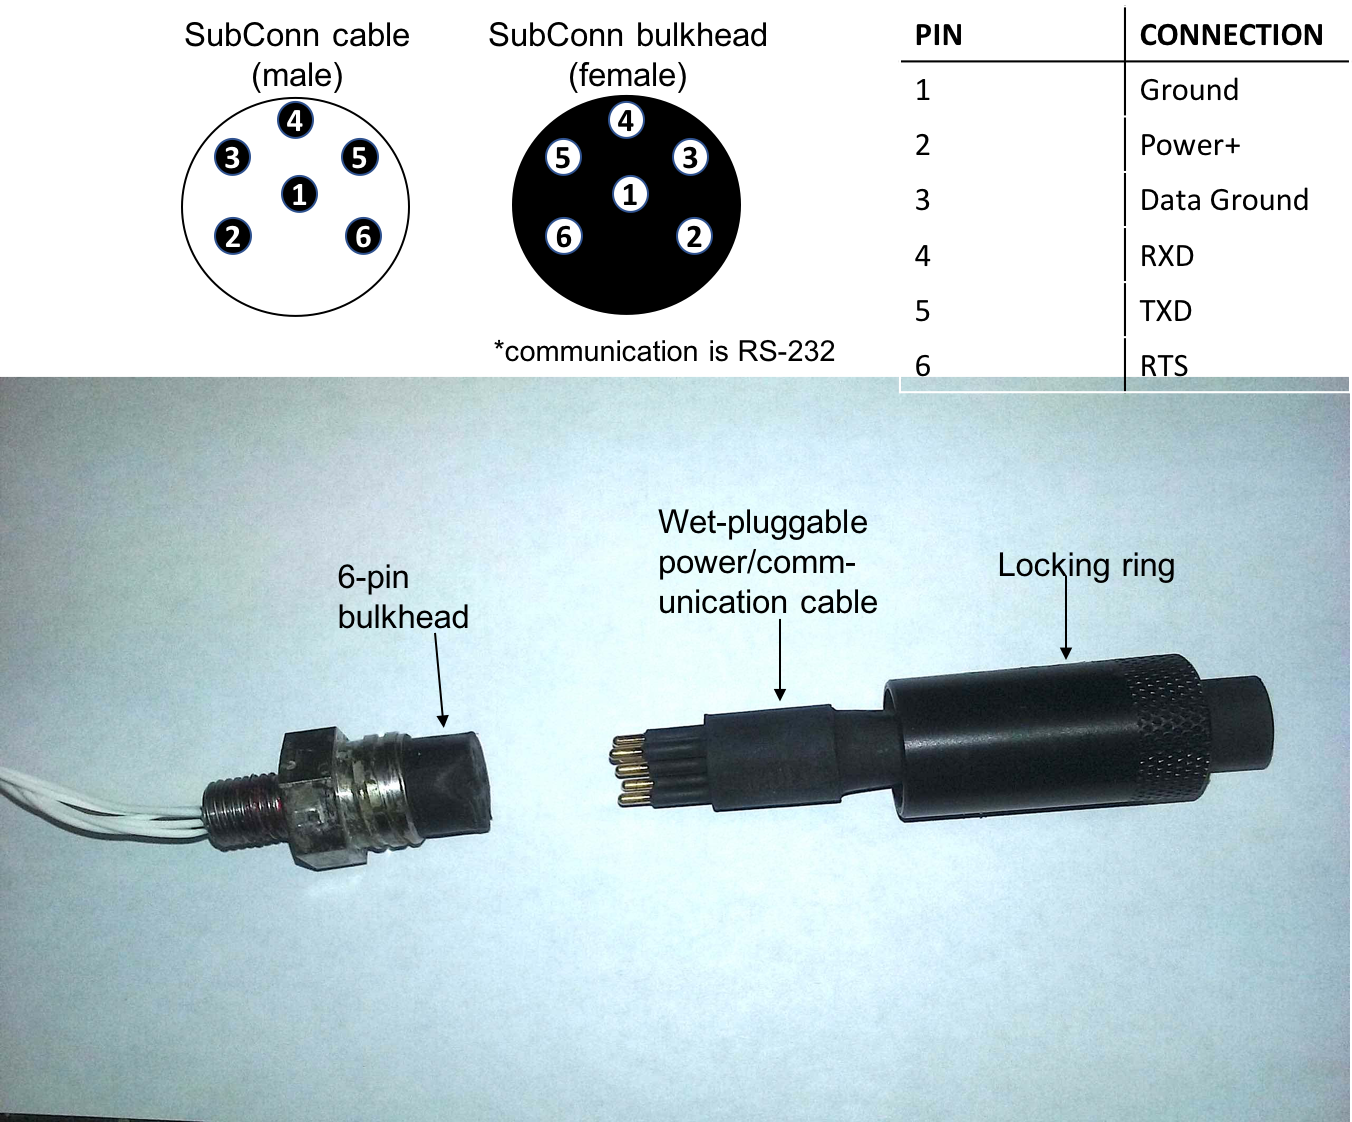
\includegraphics[width=0.8\textwidth]{figs/Subconn_cable.png}
\caption{\instType{} 6-pin connection.}
\label{fig:Subconn}
\end{figure}

\or		%AFT

The black communication cable included with your instrument will have a 6-pin connector on one end and on the other end, two diverging cables: a USB-serial converter and an AC power plug. The communication cable's bulkhead attachment should be attached to the side of your AFT instrument.  

\begin{table}[ht]
\RawFloats
\begin{minipage}[b]{0.5\hsize}
\centering
   \begin{tabular}{l l}
       \toprule
       Pin & Connection \\
       \midrule
       1 & DTR \\
       2 & RXD \\   
       3 & TXD \\
       4 & Signal GND \\
       5 & Power + \\
       6 & Power GND \\
       \bottomrule
    \end{tabular}
    \caption{Cable pin assigments.}
    \label{tab:BulginPins}
\end{minipage}
\hfill
\begin{minipage}[b]{0.5\hsize}
\centering
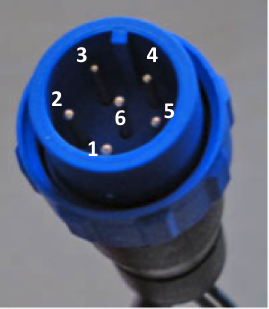
\includegraphics[scale=0.5]{figs/Bulgin_labeled.png}
\captionof{figure}{Bulgin cable connector.}
\label{fig:BulginCable}
\end{minipage}
\end{table}

\fi


\subsubsection{Communicating}

Once your instrument and computer are properly interfaced, you may start communicating with the instrument. Under \textbf{Preferences} (in the \textbf{Edit} menu for PCs, and in the \textbf{SAMI Client} menu for Macs) select the appropriate serial port. Click the \textbf{Serial Open} button to establish communication with your \instType{}. The indicator next to the Serial Port text will specify if your \instType{} is interfaced with your computer (Figure \ref{fig:InstInterface}). A red dot indicates a closed serial port while a green dot indicates an open serial port. 

Failure to connect usually indicates that the wrong port has been selected. Double check your port settings if you cannot connect. See also the troubleshooting section.

\begin{figure}[ht]
\centering
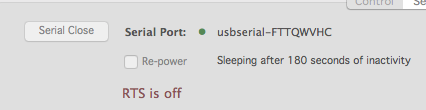
\includegraphics[width=0.6\textwidth]{figs/Inst_Interface.png}
\caption{Instrument interface.}
\label{fig:InstInterface}
\end{figure}


\subsection{Quick Start Guide}

The following procedure will guide you through the process of starting and stopping your \instType{}. A more detailed discussion can be found later in the user manual.  Please review the following checklist to ensure that the instrument is ready to start and deploy:

\begin{enumerate}
\item None of the housing compartments of your instrument have been opened since receipt. Sunburst cannot be held responsible for issues experienced if the instrument has been opened.
\item The instrument is being deployed within 90 days of receipt

\ifcase \inst	%iSAMI

\item Pump DI (deionized water in the attached bag) 30 times and check to see if liquid is coming out of the outlet tubing.
\item Remove DI Bag from inlet tubing.
\item If the instrument will be deployed through ice, remove copper bells from inlet tubing.

\or			%SAMI

\item Pump DI (deionized water in the attached bag) 30 times and check to see if liquid is coming out of the outlet tubing.
\item Remove DI Bag from inlet tubing.
\item If the instrument will be deployed through ice, remove copper bells from inlet tubing.

\or			%AFT

\fi

\item The instrument was not stored in freezing temperatures, in direct sunlight, or at high temperatures for extended periods of time.
\item If any of these points listed above were not met or if the instrument is not functioning properly prior to deployment, contact Sunburst Technical Support (techsupport@sunburstsensors.com).  Do NOT deploy instrument.
\end{enumerate}


\subsubsection{\instType{} Launch Procedure}

\begin{enumerate}

\ifcase \inst	%iSAMI

    \item Attach communication cable to \instType{}, power supply, and computer. Please note that the cable provided with the \instType{} is for bench-top programming and download of the \instType{} data.  The cable is not made for deployment, but can be used for shallow laboratory testing.
    
        \begin{enumerate}
        \item Attach the cable to the 6-pin bulk-head connection on the top of the \instType{}.
        \item Attach the banana plugs (black is ground, red is positive) to a +\,12\,VDC power supply.

        \textit{The \instType{} can be programmed for deployment in the field without a 12\,V power supply by connecting the cable to the bulkhead and to the computer.  However, the \instType{} must be connected to a 12\,V power supply \textbf{before} it begins measurements. Operation of the pump without a power supply will shut down the \instType{}.}
        
        \item Attach the USB connector to a USB port on your computer.
        \end{enumerate}
        
\or			%SAMI

    \item Attach communication cable to \instType{}, power supply, and computer. Please note that the cable provided with the \instType{} is for bench-top programming and download of the \instType{} data.  The cable is not made for deployment, but can be used for shallow laboratory testing.
    
        \begin{enumerate}
        \item Attach the cable to the 6-pin bulk-head connection on the top of the \instType{}.
        \item Attach the banana plugs (black is ground, red is positive) to a +\,12\,VDC power supply.
        \item Attach the USB connector to a USB port on your computer.
        \end{enumerate}
        
\or			%AFT

    \item Attach communication cable to \instType{}, power supply, and computer.
    
\fi    
    
    \item Install \instType{} Client software and the USB serial converter driver as described in section \ref{sec:Install}.
    
    \item The first time you run \instType{} Client, a preferences window should open allowing you to select the proper COM port.  The correct port will usually be the last one in the list on a Windows machine.  On a Mac the correct port will be \verb|usb serial Fxxxxxx| where ``x'' represents any alphanumeric character.
    
    \item If you want the application to automatically connect to the \instType{} using the same port in the future, check the box in preferences.  Dismiss the preferences dialog by clicking \textbf{OK}.
    
    \item If you did not check the box in step 4, click on the \textbf{Serial Open} button on the Control page.
    
    \ifcase \inst	%iSAMI
    
        \item Under the \textbf{Settings} tab, in the \textbf{SAMI} subpanel, choose SAMI pH (Vb+) from the dropdown menu.  \textbf{Set the desired \instType{} start time to a time at which the \instType{} will be connected to a 12\,V power supply or submersible battery pack.}  You may choose to record battery and temperature prior to start using the \textbf{Prestart} sub-panel.
        
    \else		%SAMI/AFT
    
        \item Under the \textbf{Settings} tab, in the \textbf{SAMI} subpanel, choose SAMI pH (Vb+) from the dropdown menu.  Set the desired \instType{} start time.  You may choose to record battery and temperature prior to start using the \textbf{Prestart} sub-panel.  If you have any external instruments they will be programmed using \textbf{Device 1, 2 or 3}.

    \fi
    
    \item Under the \textbf{Control} tab, click \textbf{Re-power} if Deployment Cycle Controls are not active.  Erase any data stored in the memory (download if desired), Launch!
    
    \item If you wish to watch results, you can observe output via the \textbf{Utility} tab. Under the Utility tab you can also check \instType{} status and monitor results. For more detailed output, click on the \textbf{Real Time} button. \ifcase \inst {\textbf{ Note: you must have a 12\,V power supply connected to the communication cable in order to see real-time data.}} \else \fi
    
    \ifcase \inst %iSAMI
    
        \item To exit \instType{} the Client program, click on the \textbf{Serial Close} button and then exit the program, disconnect the communication cable, and connect the \instType{} to a 12\,V power supply or submersible battery pack.  The \instType{} will continue to run as long as it is connected to power.

    \else		%SAMI/AFT
    
        \item To exit the \instType{} Client program, click on the \textbf{Serial Close} button and then exit the program, the \instType{} will continue to run.

    \fi
\end{enumerate}

\ifcase \inst	%iSAMI

    {\color{red}Before deploying the \instType{}-pH, \textbf{remove the external bag of nanopure water} when the \instType{} is \textit{not} pumping.  This is the sample inlet to the \instType{}, so failure to remove the bag will result in \textbf{no data}.  The \instType{} must then be deployed before a new sample cycle begins.  If the \instType{} begins pumping before deployment, air will be pumped into the system.  This could result in instrument failure.  If air bubbles are pumped into the system, re-attach the nanopure water bag, and run the \instType{} pump, checking that light signals are $\geq$ 6000.}

\or			%SAMI

    {\color{red}Before deploying the \instType{}-pH, \textbf{remove the external bag of nanopure water} when the \instType{} is \textit{not} pumping.  This is the sample inlet to the \instType{}, so failure to remove the bag will result in \textbf{no data}.  The \instType{} must then be deployed before a new sample cycle begins.  If the \instType{} begins pumping before deployment, air will be pumped into the system.  Depending on the depth of deployment, this could result in instrument failure.  If air bubbles are pumped into the system, re-attach the nanopure water bag, and run the \instType{} pump, checking that light signals are $\geq$ 1500.}

\or			%AFT

\fi


\subsubsection{\instType{} Stop Procedure}

\ifcase \inst	%iSAMI

\begin{enumerate}
    \item Remove \instType{} from the water and wipe down the instrument with a dry rag.
    
    \item Attach communication cable to \instType{}, power supply (12\,VDC), and computer.
    
    \item Establish communication the \instType{}.
    
    \item In the \textbf{Control} window, click on \textbf{Stop} button.
    
    \item {\color{red} Flush de-ionized water through the sample line.  You must first immerse your \instType{} in a bucket of de-ionized water or tap water that covers the inlet tube completely, or connect the inlet that protrudes from the reagent chamber, via an Upchurch 1/4--28 fitting, to a bag or beaker of de-ionized water.  If de-ionized water is not available, use tap water, but DO NOT use seawater.  Then go to the \textbf{Utility} tab, check the \textbf{Repower} box, and click on \textbf{pH Flush} on the \textbf{Cycle Pump} subpanel.}
\end{enumerate}

\or	 		%SAMI

\begin{enumerate}
    \item Remove \instType{} from the water and wipe down the instrument with a dry rag.
    
    \item Attach communication cable to \instType{}, power supply (12\,VDC), and computer.
    
    \item Establish communication the \instType{}.
    
    \item In the \textbf{Control} window, click on \textbf{Stop} button.
    
    \item {\color{red} Flush de-ionized water through the sample line.  You must first immerse your \instType{} in a bucket of de-ionized water or tap water that covers the inlet tube completely, or connect the inlet that protrudes from the brass cage, via an Upchurch 1/4--28 fitting, to a bag or beaker of de-ionized water.  If de-ionized water is not available, use tap water, but DO NOT use seawater.  Then go to the \textbf{Utility} tab, check the \textbf{Repower} box, and click on \textbf{pH Flush} on the \textbf{Cycle Pump} subpanel.}
\end{enumerate}

\or			%AFT

\begin{enumerate}
\item Re-establish communication with instrument (if necessary) by clicking on the \textbf{Serial Open} button.
\item In the Control window, click on \textbf{Stop} button.  This option is not available when the \instType{} is collecting data.
\item {\color{red} Flush de-ionized water through the sample line.  If de-ionized water is not available, use tap water, but DO NOT use seawater.  Then go to the \textbf{Utility} tab, check the \textbf{Repower} box, and click on \textbf{pH Flush} on the \textbf{Cycle Pump} subpanel.}
\end{enumerate}

\fi


\subsubsection{Real Time Data}

To view real time data click on the \textbf{Real Time Data} button. Under the \textbf{Column Set} drop-down menu, select \textbf{pH}, and then click on the \textbf{Make View Win} button. This will display the Year Day, Temperature, Battery Voltage, and pH. You can view as a Spread Sheet or Scatter Plot. 

\subsubsection{Download Data}

Once you stop the \instType{}, you can download the data by clicking on the \textbf{Download} button. The data stored on your \instType{} will be copied as a text file to a location you select on your computer. A default name of \verb|SAMI_UnitName_DDMMYY| will appear in the save dialog window. If you encounter an error while downloading, try downloading again. The data is not erased from the \instType{} until you click on the \textbf{Erase} button. To view the downloaded data, click on the \textbf{Open Data File} button in the Control window. Select the file you wish to view, and under the \textbf{Column set} drop-down menu select \textbf{pH} and then click on the \textbf{Parse File} button. Data can be viewed as a Spread Sheet or a Scatter Plot. You can export results by clicking on the \textbf{Export All Data} button.


\subsection{\instType{} Client Interface}

\instType{} Client is the interface for your instrument, both \instType{} and \instType. The \textbf{SAMI Client} menu is divided into three different tabs to help you organize the information that you will be communicating to your instrument. 

The \textbf{Control Tab} is where you will find buttons that manage basic operations such as establishing communication, downloading and erasing data, as well as launching and stopping the instrument.

The \textbf{Settings Tab} is where the deployment parameters and settings will be configured. The start time, interval between measurements, and any external device settings are set here. 

The \textbf{Utility Tab} contains an interactive display that shows live data being collected. There are also controls that will allow you to create a pumping cycle so you can easily flush the instrument.


\subsubsection{File Menu}

\begin{itemize}
    \item[] \textbf{Open Data File:} Imports data files for data processing.
    
    \item[] \textbf{Import Hex File:} Imports data that was stored by custom user systems in hex format.
    
    \item[] \textbf{Import Settings from File:} Loads previously saved launch settings that have been created under the Settings Tab. This feature will save you time once you have decided upon your customized launch settings. 
    
    \item[] \textbf{Save Settings As...:} Stores launch settings from your Settings Tab so they may be easily loaded at a later time. The \textbf{Import Settings from File} option will load these settings which you have chosen under the SAMI Box in the \textbf{Settings} tab.
    
    \item[] \textbf{Exit (PC only):} Shuts down \instType{} Client Software. This does not disrupt \instType{} operation. This function is located in the \textbf{SAMI\_Client} menu on a Mac.
    
    \item[] \textbf{About... (PC only):} Software credits and version number displayed in dialogue window. This function is located in the \textbf{SAMI\_Client} menu on a Mac.
\end{itemize}


\subsubsection{Edit Menu}

The \textbf{Preferences} tool under this heading (PC only) is important for communication with your instrument. If using a Mac, \textbf{Preferences} is found under \textbf{SAMI\_Client} menu. \textbf{Preferences} contains a dropdown menu that is populated with the serial ports on your computer. To communicate successfully with your \instType{}, the correct serial port must be selected. If the correct serial port is not present in the list, you may need to wait for the rest of the ports to be identified. Check the \textbf{Auto-Open serial port} box to automatically establish communication with your \instType{} once the correct serial port has been selected. You will also set your \instType{} to default to either Local Time or GMT on the \textbf{Preferences} page.


\subsubsection{SAMI Menu}

\begin{itemize}
    \item[] \textbf{Read SAMI Settings:}
    The SAMI Launch Setting programmed into your \instType{} can be viewed by choosing this option. A separate window will appear with the Settings displayed in list format.  This option is only active if the \instType{} is \textbf{NOT} running \textbf{AND} the \textbf{Port Powered} box is checked on either the \textbf{Control} or \textbf{Utility} tab.
    
    \item[] \textbf{Read/Edit SAMI Text:}
    The text added to the \instType{} under the \textbf{Edit Text} button on the control tab can be viewed by selecting this option. This option is only active if the \instType{} is \textit{NOT} running \textit{AND} the \textit{Port Powered} box is checked on either the control or utility page.
    
    \item[] \textbf{Update Firmware:}
    This action will be performed when software updates become available through Sunburst Sensors.  As you receive or download newer versions of the \textbf{SAMI\_Client}, upgrades to the firmware may accompany these.  If required, an advisory message suggesting update of the firmware will appear when you first connect to the \instType{}.
    
    \begin{figure}
    \centering
    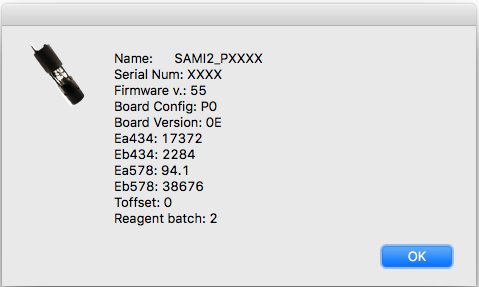
\includegraphics[width=0.6\textwidth]{figs/Cal_Info.png}
    \caption{Read calibration window.}
    \label{fig:CalInfo}
    \end{figure}
    
    \item[] \textbf{Read Cal Info:} Figure \ref{fig:CalInfo} lets you view E values, \instType{} temperature offset compared to NIST-traceable standard, and reagent type (1 is un-purified; 2 is purified). These values should match the values on the calibration certificate that was shipped with the \instType{} after the most recent refurbishment.  If values do not match, contact Sunburst Sensors before deployment.
\end{itemize}


\subsubsection{Help Menu}

Various documents are available via the Help menu, including this manual, release notes for the software detailing what changes have been made, use of external instruments, etc.

\begin{itemize}
    \item[] \textbf{View Sunburst Website:}
    This heading will direct you to \url{http://www.sunburstsensors.com} for convenient access to our business, research, and contact information. 
    
    \item[] \textbf{Send us Email:}
    Directs email to Info@sunburstsensors.com
    
    \item[] \textbf{About SAMI application (PC):}
    Brings up an information and credits window.
    
    \item[] \textbf{Check for Updates:}
    If you have an internet connection the \instType{} Client software will automatically check the Sunburst Sensors website for updates to the software upon launch. You can manually check via this menu item.
\end{itemize}


\subsubsection{Control Tab}

The \textbf{Control} tab is where you establish communication and power with the \instType{}, start and stop sample collection, and download data.

\begin{figure}[ht]
\centering
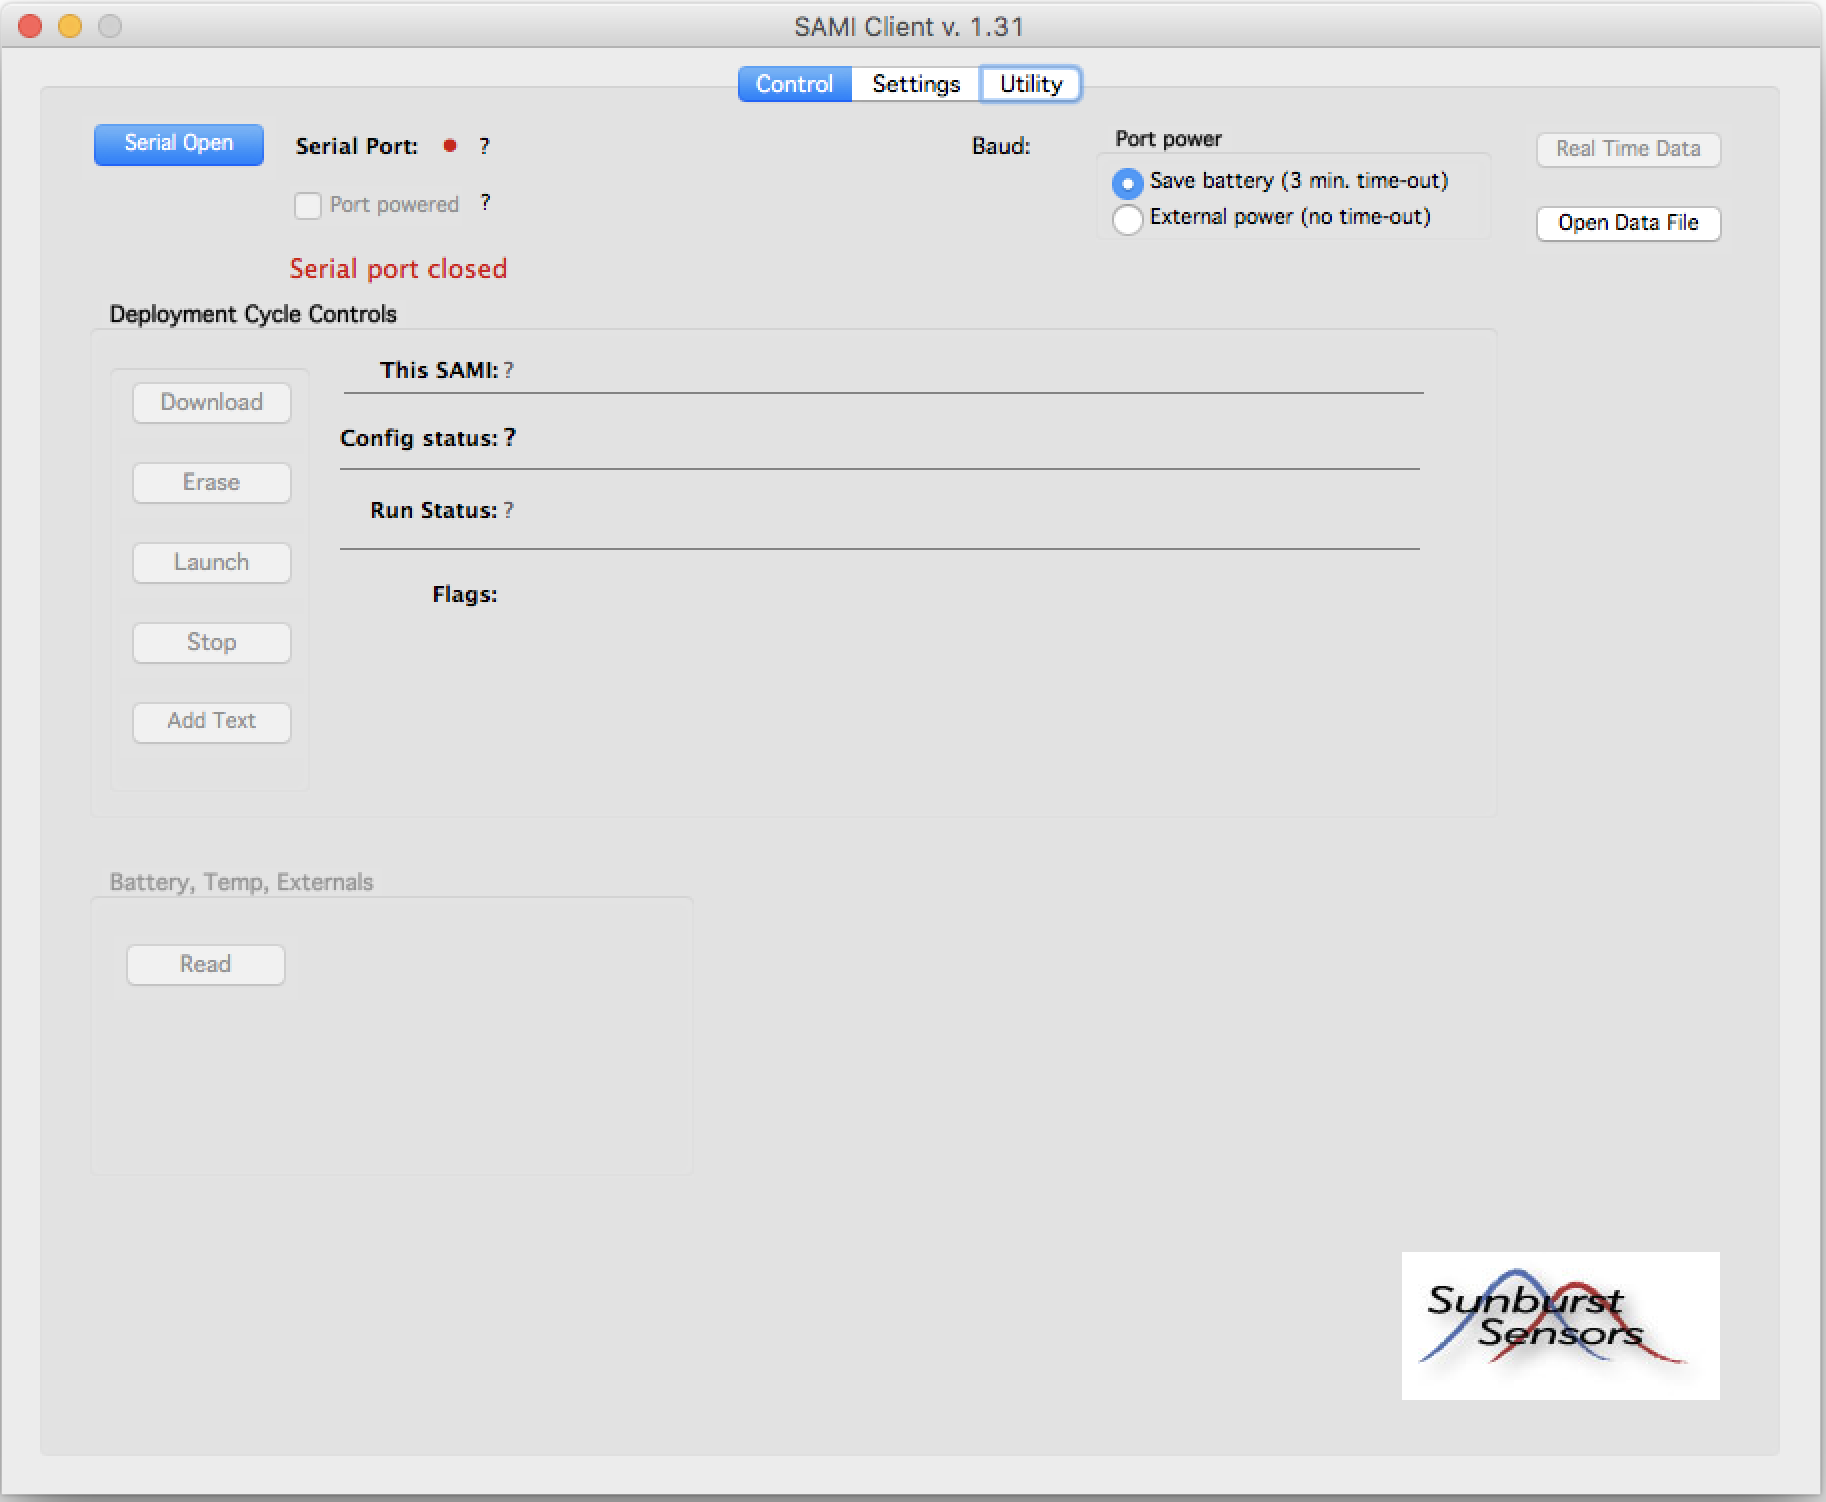
\includegraphics[width=1.0\textwidth]{figs/Cntl_Tab.png}
\caption{Control tab.}
\label{fig:CntlTab}
\end{figure}


\subsubsection{Serial Communication}
\label{Serial}

The \textbf{Serial Open/Serial Close} button engages \textbf{SAMI\_Client} to communicate with your instrument. To establish communication, attach the communication cable to your computer and \ifcase \inst {\instType{}, and power to 12\,V supply or battery.} \or {\instType{}.} \or {and power \instType{}.} \fi In Edit $\rightarrow$ Preferences (PC), or SAMI Client $\rightarrow$ Preferences (Mac) select the appropriate serial port. Click the \textbf{Serial Open} button to begin communication with your \instType{}. The indicator next to the Serial Port text will specify if your \instType{} is interfaced with your computer. A red dot indicates a closed serial port while a green dot indicates an open serial port (Figures \ref{fig:InstInterface} and \ref{fig:CntlTab}). 

If the \textbf{Auto-Open Serial } box is checked in the \textbf{Preferences} pop-up page, the \textbf{Serial Open/Serial Close} button will no longer be visible and the \instType{} will automatically try to establish communication when it is powered on.

\begin{figure}[ht]
\centering
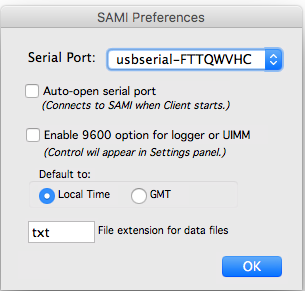
\includegraphics[width=0.5\textwidth]{figs/Prefs.png}
\caption{Communication preferences pop-up window}
\label{fig:Prefs}
\end{figure}


\subsubsection{Power Settings}
\label{sec:SoftwarePower}

\begin{itemize}
    \item[] \textbf{Port Powered/Re-power:}
    You can communicate with the \instType{} and program it for deployment without connecting to external power.  To conserve the small internal battery, the  communications will time out after 3 minutes, unless you override this feature by selecting the \textbf{External Power} radio button. If the port does time out, you can re-open it by simply clicking the \textbf{Re-power} check box. If communications has timed-out, you cannot send commands or program the \instType{} until the port is re-powered.
    
    If the \instType{} is \ifcase \inst {running (while connected to 12\,V power),} \else {running,} \fi however, the  will send data out over the serial port after each measurement or other event, even if the port is timed out (The \instType{} powers up the port just long enough to send data).
    
    \item[] \textbf{Save Battery:}
    The Save battery option should be selected when not connected to external power. This allows the \instType{} to go into time-out after three minutes and preserves the internal battery. This function may also be controlled from the \textbf{Utility} tab.
    
    \item[] \textbf{External power:}
    If the \instType{} is connected to a 12\,VDC power supply, you can select this option to keep communication open with the \instType{} Client at all times. If \textbf{External Power} is selected, the message \say{Port power on until disconnected} will appear under serial port. This function may also be controlled from the utility tab.
\end{itemize}


\subsubsection{Deployment Cycles Controls Panel} 

\begin{itemize}
    \item[] \textbf{Download}
    The \textbf{Download} button will copy data stored on your \instType{} to a location you select on your computer.  A default file name of \verb|SAMI_UnitName_DDMMYY| will be suggested in the save dialog. Data will not be erased from the \instType{} by using the Download function.  If download fails, try it again.
    
    \item[] \textbf{Erase:}
    The \textbf{Erase} button will clear the memory on the \instType{} of the data that it previously collected. To launch your \instType{} you must erase all data stored on the \instType{}. If you wish to save the data from your last data collection you MUST download the information before it is erased. If you attempt to erase data before it has been downloaded, you will get a warning message \say{Data has not been downloaded!} \textbf{OK} will erase all data and settings! 
    
    \item[] \textbf{Add Text:}
    The \textbf{Add Text} button allows you to add notes to the instruments memory. The notes will be displayed in the data output files and can be accessed from the Toolbar SAMI $\rightarrow$ Read SAMI Text.  
    
    \item[] \textbf{Launch}
    \label{Launch:}
    Unless the \instType{} has been erased, it cannot be launched. Prior to launch, use the controls in the Settings Tab to configure the \instType{}; setting the start time, sample interval, etc.  
    If you have set a launch time that has passed, you will get the message \say{Start is less than 10 seconds from now!  Would you like to start in 10 seconds?}. This may be OK for bench-top testing, but if you require data aligned to the hour, you should program the start time accordingly.
           
    \item[] \textbf{Stop:}
    The \textbf{Stop} button will end the launch of your instrument and sampling will cease. Data will be saved in the memory of your instrument.
\end{itemize}


\subsubsection{Configuration status Panel} 

\begin{itemize}
    \item[] \textbf{Serial Port Opened:}
    \label{Serial}
    The \instType{} has established communication with your computer. 
    
    \item[] \textbf{Config loaded and \instType{} started:}
    Indicates that your program has launched and measurement collection has begun.
    
    \item[] \textbf{(\#:) of Pages downloaded}
    This message appears when a measurement sequence has been stopped and you have downloaded a file. 
    
    \item[] \textbf{Erased:}
    The memory has been cleared and you may begin another measurement sequence.
\end{itemize}


\subsubsection{Flags}

The Flags section will display messages that indicate status:
 
This \instType{}: \quad Name: \quad SN: \quad Hardware: \quad Firmware:

\begin{itemize}
    \item[] \textbf{Recording Started:}
    Data is being collected and stored in your instrument's memory.
    
    \item[] \textbf{Recording Stopped:}
    The measurement sequence has stopped. The data has not yet been downloaded or erased.
    
    \item[] \textbf{Downloaded:}
    The measurement sequence has been stopped.  The data has been downloaded, but not erased. Erase your data before continuing with another sequence of measurements.   
    
    \item[] \textbf{Run Status:}
    
    While the program is running, the Run Status will display the date, time, number of data files collected, and the memory used. The Run Status section will remain blank if the program is not running, the files have been downloaded, or the data file is erased.
\end{itemize}


\subsubsection{Battery, Temp, Externals Panel}

\begin{wrapfigure}[4]{r}{0.6\textwidth}
\centering
\vspace{-5mm}
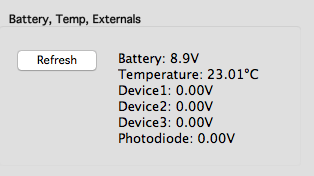
\includegraphics[width=0.8\textwidth]{figs/Read_Batt.png}
\caption{Battery, Temperature, Externals panel}
\label{fig:ReadBatt}
\end{wrapfigure}

Clicking the \textbf{Read} button updates information on the battery voltage, the temperature in Celsius, and the output voltage of any external devices.

\vspace{30mm}


\subsubsection{Settings Tab}

\paragraph{Overview}
The \textbf{Settings} tab contains the various control panels used to configure the instrument prior to a deployment. These control panels allow the user to set the start time and run duration, sampling interval, etc. It is important to note that these settings are not sent to the instrument until the user launches the unit via the \textbf{Launch} button in the deployment controls (section \ref{Launch}).  

\begin{figure}[h]
\centering
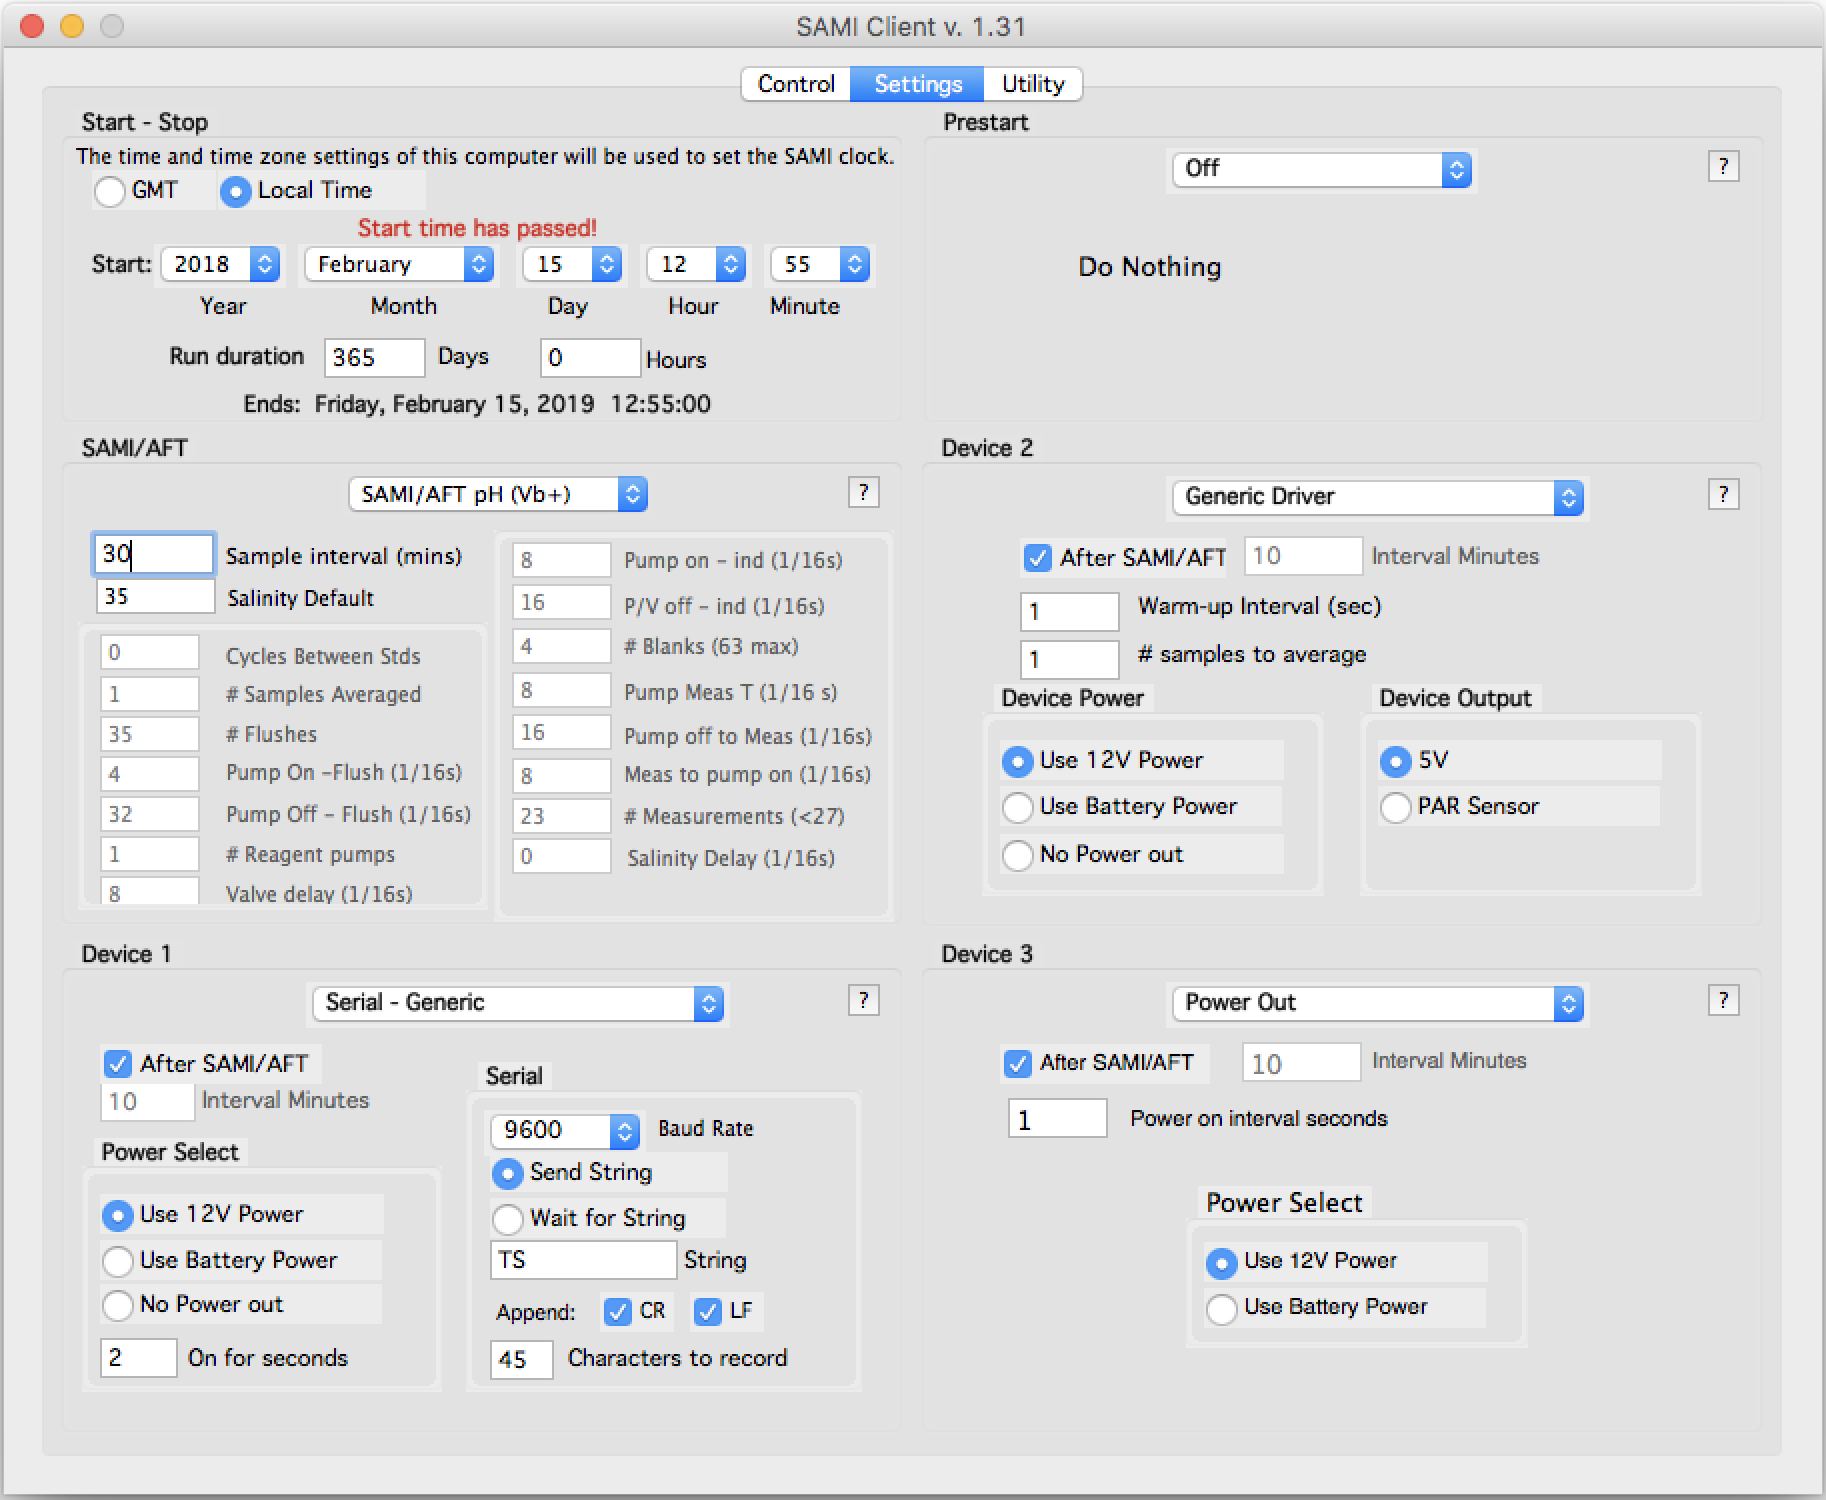
\includegraphics[width=1.0\textwidth]{figs/Set_Tab2.png}
\caption{Settings tab.}
\label{fig:SetTab2}
\end{figure}


\subsubsection{Start-Stop Panel}

In the \textbf{Start-Stop} panel in the upper left hand corner of the \textbf{Settings} tab you will enter your deployment start time and the run duration. You may enter the exact time you wish to launch your instrument, accurate to five minutes. Note that you may display your time in GMT or local time. However, \textbf{data is stored on the \instType{} in GMT, regardless of the time format set here.} When you enter the run duration in the specified box, a message appears below which will calculate the end time and date. 

In the event that the start time has passed, you will receive a message informing you the start time has passed. When you Launch your instrument a message box will ask if you wish to begin sampling in ten seconds.  By selecting \textbf{OK} measurements will begin immediately. Otherwise you may select a new start time by selecting \textbf{Cancel}.


\subsubsection{SAMI/AFT Panel}

The \textbf{SAMI/AFT} panel is where you will enter the sampling interval. In the dropdown menu in the top center of the box, select \textbf{SAMI-pH (Vb+)}. The sample interval must be entered in minutes and with a time of no less than five minutes (15\,min is optimal).  Enter the approximate or measured salinity of the sample in \textbf{Salinity Default}.  This salinity will be used to calculate \pKa for the pH measurement.  The grayed-out controls on the right hand side of the control panel are not user adjustable, but visible for trouble shooting and support.


\subsubsection{External Device Panels}

\ifcase \inst	%iSAMI

External devices are not supported by the \instType{}.

\else			%SAMI/AFT

The \instType{} supports up to three external devices, such as PAR sensors, fluorimeters, dissolved oxygen optode, or similar. It can read and log device output. It will support one RS232 serial device and two 0--5\,VDC output devices, or three 0--5\,VDC devices with no serial device. These devices can be scheduled with reference to the \instType{}'s own measurements, occurring immediately after the measurement has completed, or on a set interval.

Contact Sunburst if you wish to control an external device with the \instType{}. The \instType{} is not configured to support external devices in the base model (there is no wiring to support the externals).

\paragraph{Generic Driver}
The generic driver supports 0--5\,VDC input. Select the scheduling of the device by specifying whether to activate after the \instType{} measurement or at a fixed interval. The \textbf{Warm-Up Interval} allows the external device to stabilize before measuring and should be set in accordance with manufacturers suggestions. The \textbf{\# samples to average} allows multiple readings to be averaged. The power selection allows devices that have their own power conditioning to access the instrument batteries directly and thereby increase efficiency.  Some devices, such as a PAR sensor, require no power.  Other options include generic serial, serial, devices, etc.

\fi


\subsubsection{Utility Tab}

\begin{figure}[ht]
\centering
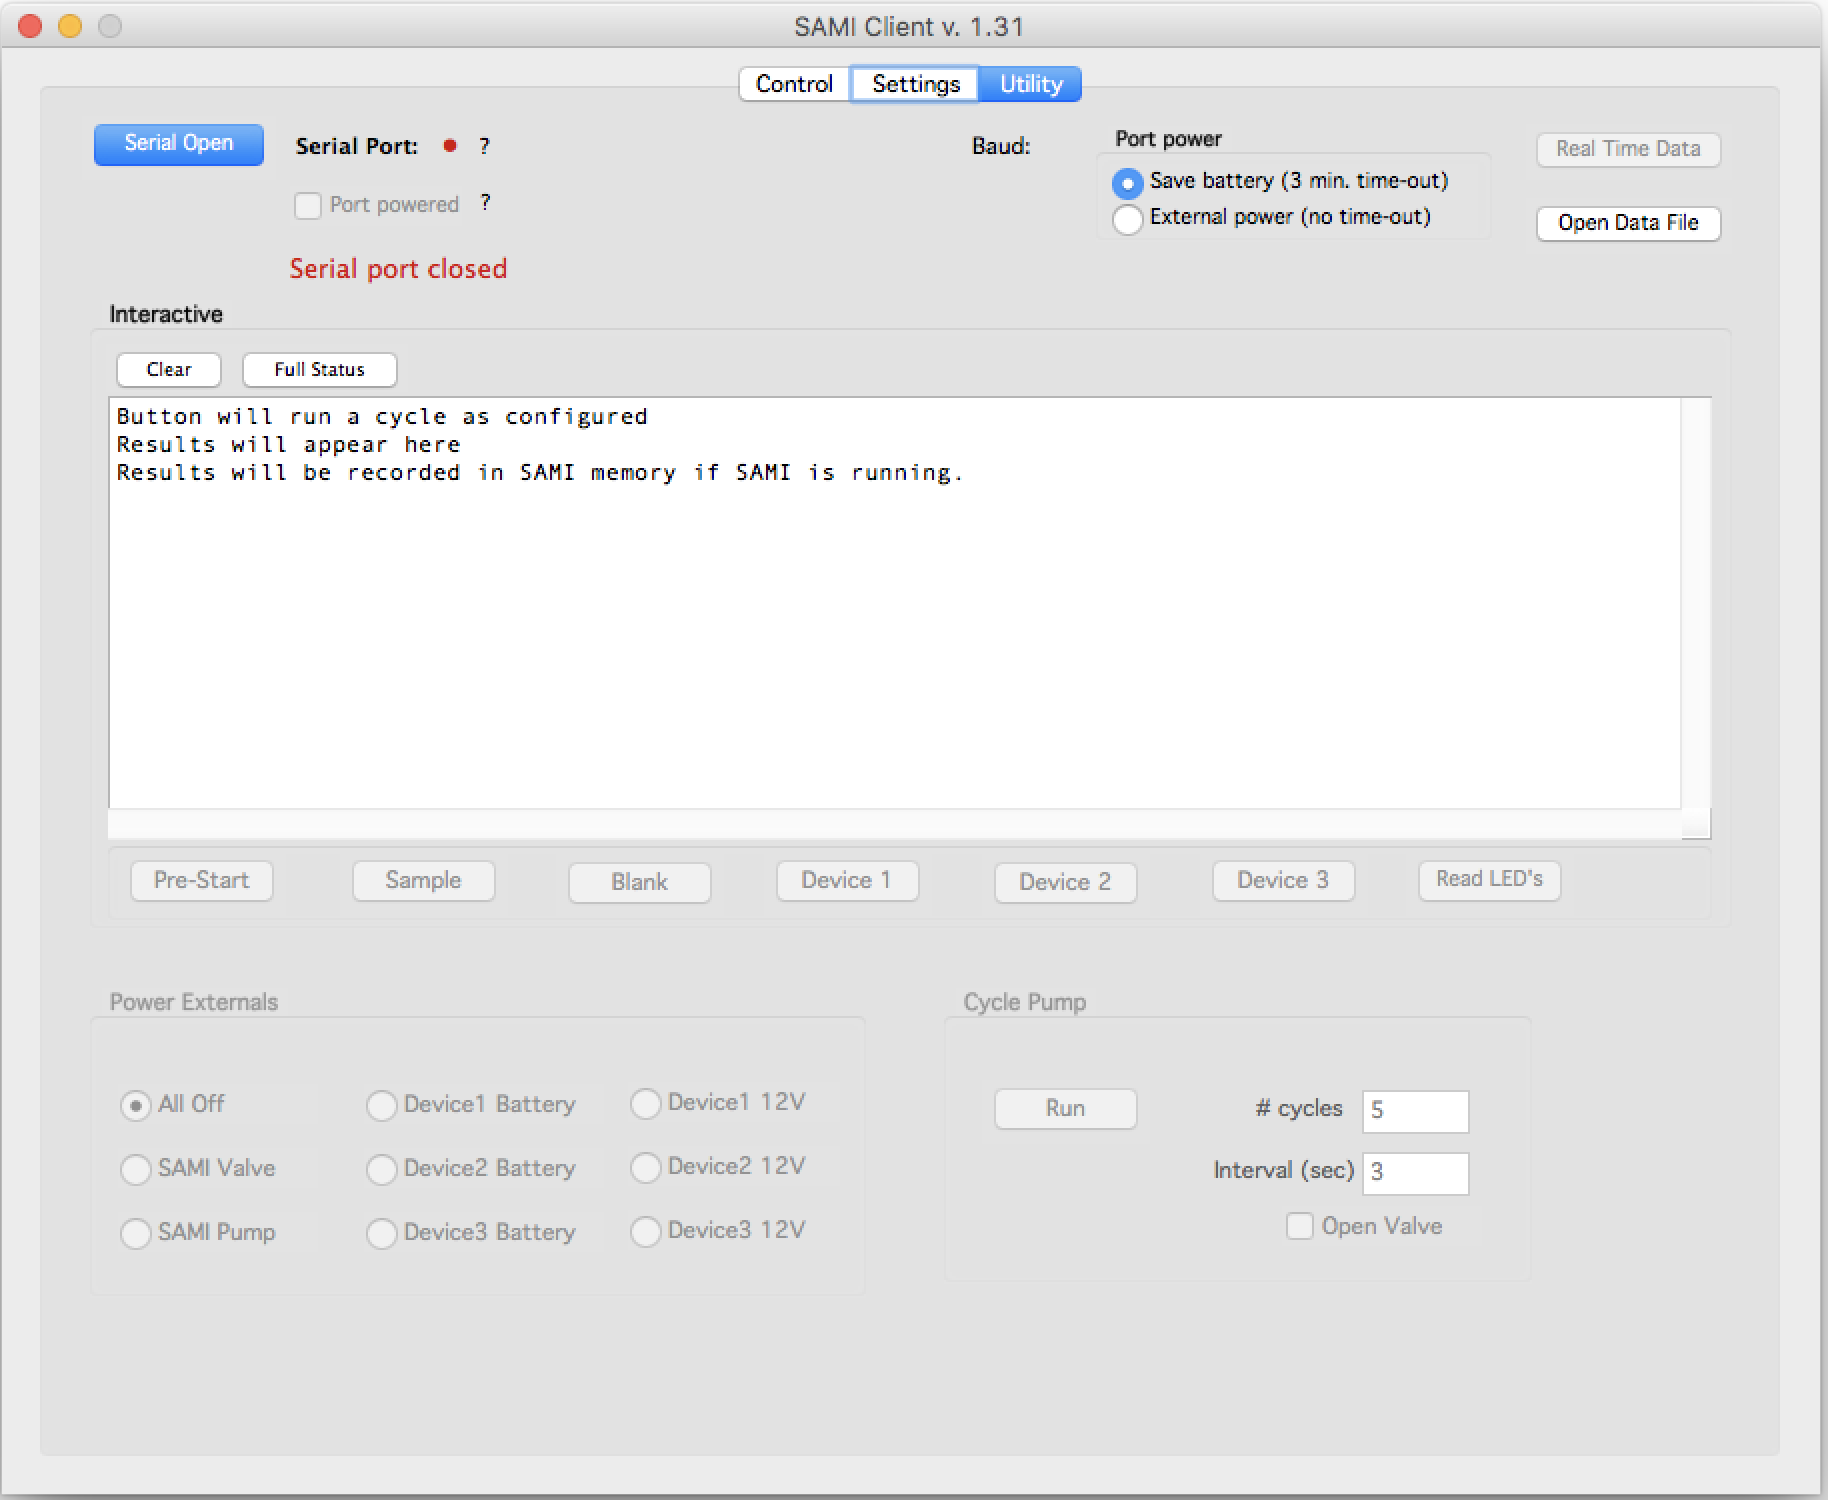
\includegraphics[width=1.0\textwidth]{figs/Util_Tab.png}
\caption{Utility tab.}
\label{fig:UtilTab}
\end{figure}

The \textbf{Utility} tab is generally used for trouble-shooting, to flush the \instType{} prior to storage or at the end of a deployment, and for data processing.


\subsubsection{Serial Port Open-Close, Port Power}

These functions can be controlled from the \textbf{Control} tab or from the \textbf{Utility} tab. See explanation of their functions in section \ref{Serial}.


\subsubsection{Interactive}

\ifcase \inst	%iSAMI

The \textbf{Interactive} panel will give you live feed on the data that your instrument is collecting when the communication cable is connected to 12\,V power. With each measurement, a string of information is written to the window. The first line will start with \say{Launch.} The next line will have the headers for the following columns of data: sample type, yearday, initial internal temperature, $\textrm{(434\,nm reference, 434\,nm signal, \linebreak 578\,nm reference, 578\,nm signal)}_n$, final internal temperature, battery voltage, external temperature. All readings are 14-bit. $n$ is \# Blanks plus \# Measurements from the Settings; default is 27. Data will be written to the screen each time a measurement is taken. This information is mostly for trouble-shooting. The records are not processed (i.e. pH, etc. is not calculated). At the top of the display you will notice a button marked \textbf{Clear} which will clear the display. The \textbf{Clear} button will not erase data from the memory.

\or			%SAMI/AFT

The \textbf{Interactive} panel will give you live feed on the data that your instrument is collecting. With each measurement, a string of information is written to the window. The first line will start with \say{Launch.} The next line will have the headers for the following columns of data: sample type, yearday, initial internal temperature, $\textrm{(434\,nm reference, 434\,nm signal, \linebreak 578\,nm reference, 578\,nm signal)}_n$, final internal temperature, battery voltage, external temperature. All readings are 12-bit. $n$ is \# Blanks plus \# Measurements from the Settings; default is 27. Data will be written to the screen each time a measurement is taken. This information is mostly for trouble-shooting. The records are not processed (i.e. pH, etc. is not calculated). At the top of the display you will notice a button marked \textbf{Clear} which will clear the display. The \textbf{Clear} button will not erase data from the memory.

\fi

\begin{itemize}
    \item[] \textbf{Read LEDs:}
    The \textbf{Read LEDs} button allows the user to check the Reference and Signal intensities of the instrument.  This can help alert the user to problems such as a blocked flow cell path or malfunctioning valve and can otherwise help to ensure the instrument is ready to deploy.
    
    \item[] \textbf{Pre-Start:}
    The instrument can be programmed to perform functions while it is waiting to start.  If this has been configured, it will read battery and temperature as programmed in the Pre-start section of the \textbf{Control} tab.
    
    \item[] \textbf{Sample:}
    The \textbf{Sample} button will run a measurement according to your programmed specifications. The measurement will not be saved in your stored data but will display in the \textbf{Interactive} panel unless the instrument has been launched.
    
    \item[] \textbf{Device 1, 2, 3:}
    \ifcase \inst	%iSAMI
    
    External devices are not supported by the \instType{}.
    
    \or			%SAMI/AFT

    This will take a reading of the device selected.  The data will not be saved in your stored data but will display in the \textbf{Interactive} panel.
    
    \fi
\end{itemize}


\subsubsection{Power Externals}

\ifcase \inst	%iSAMI

The \textbf{Power External} buttons located beneath the Interactive screen and can power the pump or valve, or an external device using 12\,VDC or battery voltage. External devices are not supported by the \instType{}. 

\or			%SAMI

The \textbf{Power External} buttons located beneath the Interactive screen and can power the pump or valve, or an external device using 12\,VDC or battery voltage.  This is useful for testing and running a CTD that is powered by the \instType{}.

\or			%AFT

The \textbf{Power External} buttons located beneath the Interactive screen and can power the pump or valve, or an external device using 12\,VDC.  This is useful for testing and running a TSG that is powered by the \instType{}.

\fi


\subsubsection{Cycle Pump}

The \textbf{Cycle Pump} function is available to flush your instrument. Flushing is an important function for the health of your \instType{} as well as to maintain a clear optical path. To flush the pH \instType{} you will need to attach the small fluid bag that came with the \instType{} or submerge the inlet tubing in deionized water, and click on \textbf{pH Flush}. The instrument will need to be flushed after each deployment in seawater.  \textit{Do not} check the \textbf{Open Valve} box, as this will flush the instrument with reagent.

The \textbf{Open Valve} box will initiate the valve during the pumping cycle. By checking this box, the initiation of the valve will pump reagent in your \instType{}-pH. The \textbf{\# cycles} refers to the number of \ifcase \inst {25\,$\mathrm{\mu L}$} \else {50\,$\mathrm{\mu L}$} \fi pumps you wish to flush through the instrument. You may choose up to 99. \textbf{Interval (secs)} refers to the amount of time between each \ifcase \inst {25\,$\mathrm{\mu L}$ pump (1\,s or greater).} \else {50\,$\mathrm{\mu L}$ pump (1\,s or greater).} \fi


\subsection{Viewing Data}

\ifcase \inst	%iSAMI

Data can be viewed in real time or imported from a file after download. On the \textbf{Control} or \textbf{Utility} tab the \textbf{Read Real Time} button becomes activated when the software detects a new measurement record (if you have connected to a \instType{} that is already running) or immediately after the \textbf{Launch} button is pushed. Data that has been previously downloaded can be imported by selecting the \textbf{Open Data File} button or selecting \textbf{Import Data File} from the File menu. The \instType{} must be powered with a 12\,VDC supply in order to view realtime data.

\else			%SAMI/AFT

Data can be viewed in real time or imported from a file after download. On the \textbf{Control} or \textbf{Utility} tab the \textbf{Read Real Time} button becomes activated when the software detects a new measurement record (if you have connected to a \instType{} that is already running) or immediately after the \textbf{Launch} button is pushed. Data that has been previously downloaded can be imported by selecting the \textbf{Open Data File} button or selecting \textbf{Import Data File} from the File menu.

\fi

\begin{itemize}
    \item[] \textbf{Data Overview:}
    Raw \instType{} data is stored as records while the \instType{} is running. These same records are transmitted over the serial port as well, so the client software will recognize and interpret them in real time.
    
    \item[] \textbf{Raw Record Structure:}
    There are two main types of records recorded by the instrument. There are data records and information records.  Every record leads with an identifying number (Record Type) and a 4-byte time stamp. Information records note events such as start, stop, low battery and possible errors if one should occur. Data records follow the type/time fields with a series of fields composed of the various readings (e.g. temperature, dark signal) needed for the measurement.  In raw format these readings are not especially informative except in trouble-shooting situations.
    
    \item[] \textbf{Computed fields:}

    \ifcase \inst	%iSAMI
    
    Computed fields consist of data derived from the raw records. For example, the raw thermistor reading is stored as a 14-bit number (0--16384). The temperature field is the temperature calculated from that raw number. Time is stored as a 4-byte number reflecting total seconds since Jan 1, 1904, while calculated fields allow time to be displayed in a variety of formats.
    
    \else		%SAMI/AFT
    
        Computed fields consist of data derived from the raw records. For example, the raw thermistor reading is stored as a 12-bit number (0--4095). The temperature field is the temperature calculated from that raw number. Time is stored as a 4-byte number reflecting total seconds since Jan 1, 1904, while calculated fields allow time to be displayed in a variety of formats.
    
    \fi
    
    \item[] \textbf{Viewing real time data:}
    
    \ifcase \inst	%iSAMI
    
     The \textbf{Real Time Data} button plots data that is being collected by the instrument in real time. When you click on the \textbf{Real Time Data} button, a pop-up with a drop down menu titled Column Set will appear. \instType{} Client has a number of previously compiled parameter sets that you can choose from in Column Set Lists. Choose \textbf{pH$\_$ConstSal}. Be sure that the approximate salinity is entered in \textbf{Salinity Default} on the \textbf{Settings} tab. A new window will open with data in spreadsheet format. A drop down menu titled Display Type allows you to view data in spreadsheet or scatter plot format.

    \or			%SAMI
    
      The \textbf{Real Time Data} button plots data that is being collected by the instrument in real time. When you click on the \textbf{Real Time Data} button, a pop-up with a drop down menu titled Column Set will appear. \instType{} Client has a number of previously compiled parameter sets that you can choose from in Column Set Lists. Choose \textbf{pH$\_$ConstSal} if you did not measure salinity with a CTD that was controlled by the \instType{}.  Be sure that the approximate salinity is entered in \textbf{Salinity Default} on the \textbf{Settings} tab.  Choose \textbf{pH$\_$MeasSal} if the \instType{} logged data from a CTD. Select \textbf{Make View Win} to view the data. A new window will open with data in spreadsheet format. A drop down menu titled Display Type allows you to view data in spreadsheet or scatter plot format.

    \or			%AFT
      The \textbf{Real Time Data} button plots data that is being collected by the instrument in real time. When you click on the \textbf{Real Time Data} button, a pop-up with a drop down menu titled Column Set will appear. \instType{} Client has a number of previously compiled parameter sets that you can choose from in Column Set Lists. Choose \textbf{pH$\_$ConstSal} if you did not measure salinity with a TSG that was controlled by the \instType{}.  Be sure that the approximate salinity is entered in \textbf{Salinity Default} on the \textbf{Settings} tab.  Choose \textbf{pH$\_$MeasSal} if the \instType{} logged data from a TSG. Select \textbf{Make View Win} to view the data. A new window will open with data in spreadsheet format. A drop down menu titled Display Type allows you to view data in spreadsheet or scatter plot format.
    
    \fi
    
    \begin{figure}[!h]
    \centering
    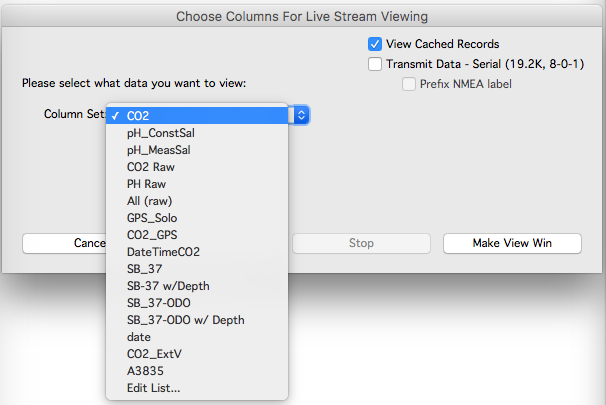
\includegraphics[width=0.5\textwidth]{figs/Real_Time.png}
    \caption{Real-time data dropdown menu.}
    \label{RealTime}
    \end{figure}
    
    \item[] \textbf{Spreadsheet:}
    The Spreadsheet format will allow you to view the data being collected as a list (Figure \ref{fig:ProcData}). 
    \vspace{5mm}
    
    \begin{figure}[!h]
    \centering
    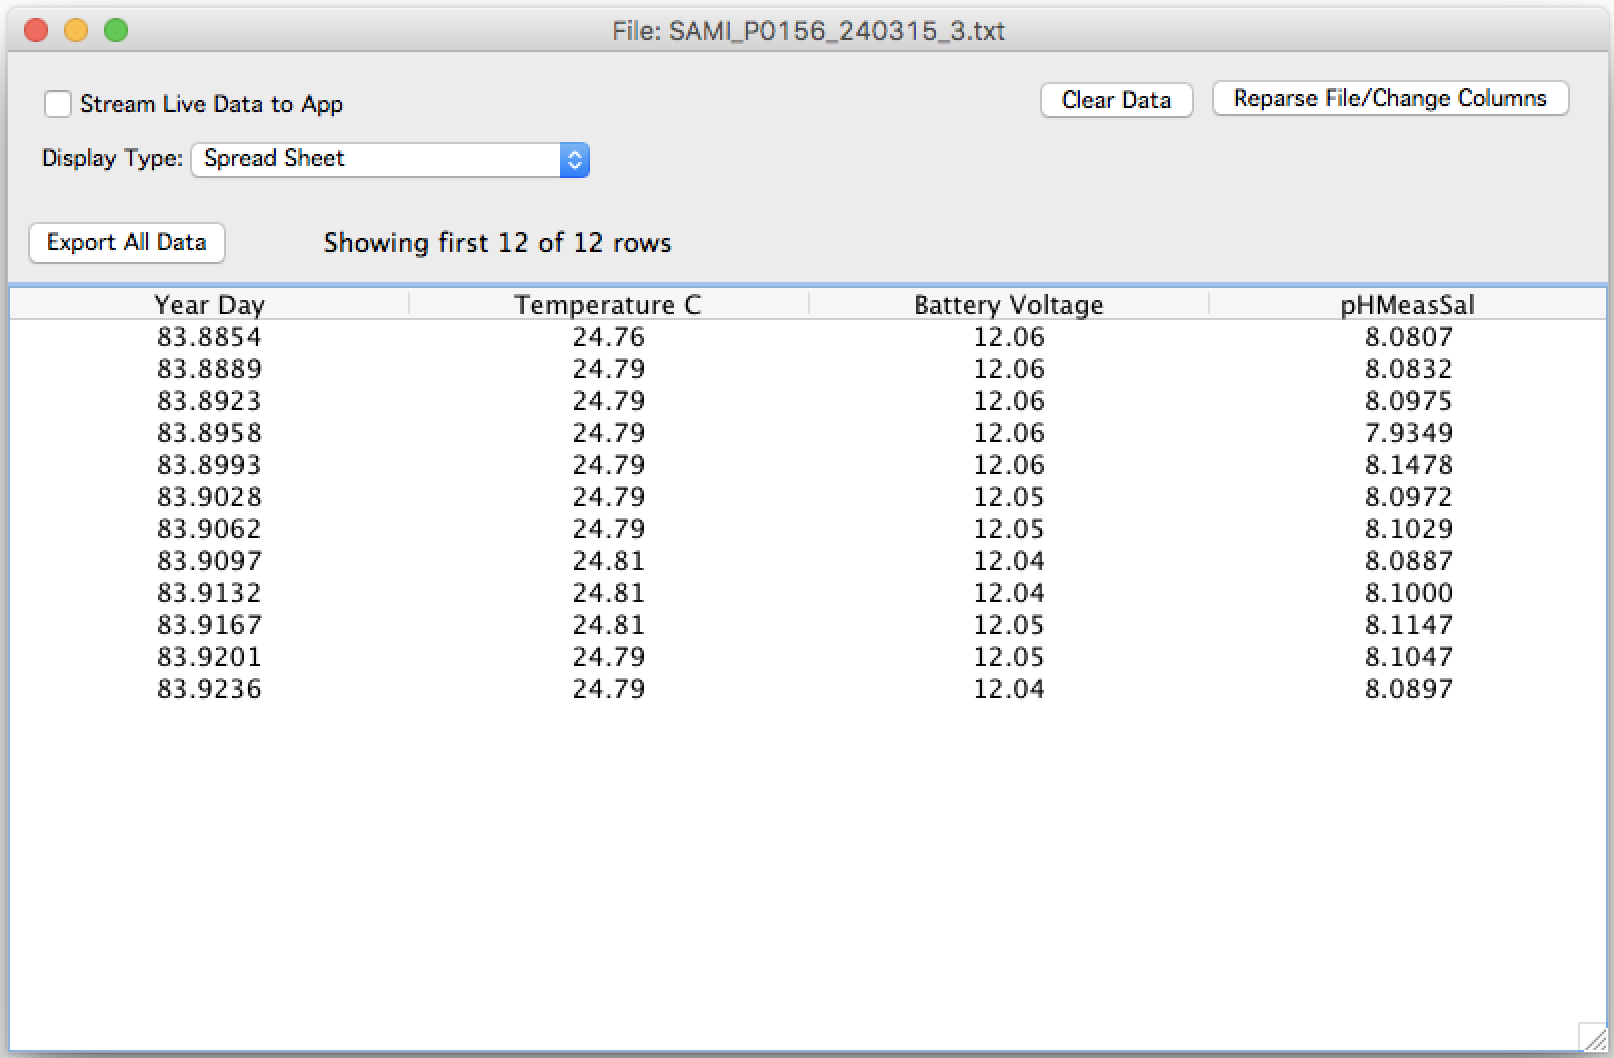
\includegraphics[width=0.7\textwidth]{figs/Proc_Data.png}
    \caption{Processed data in spreadsheet format.}
    \label{fig:ProcData}
    \end{figure}
    
    \item[] \textbf{Scatter Plot:}
    Under the Scatter Plot data display select the x-axis and y-axis parameters you wish to plot (Figure \ref{fig:PlotData}). 
    
    \begin{figure}[!h]
    \centering
    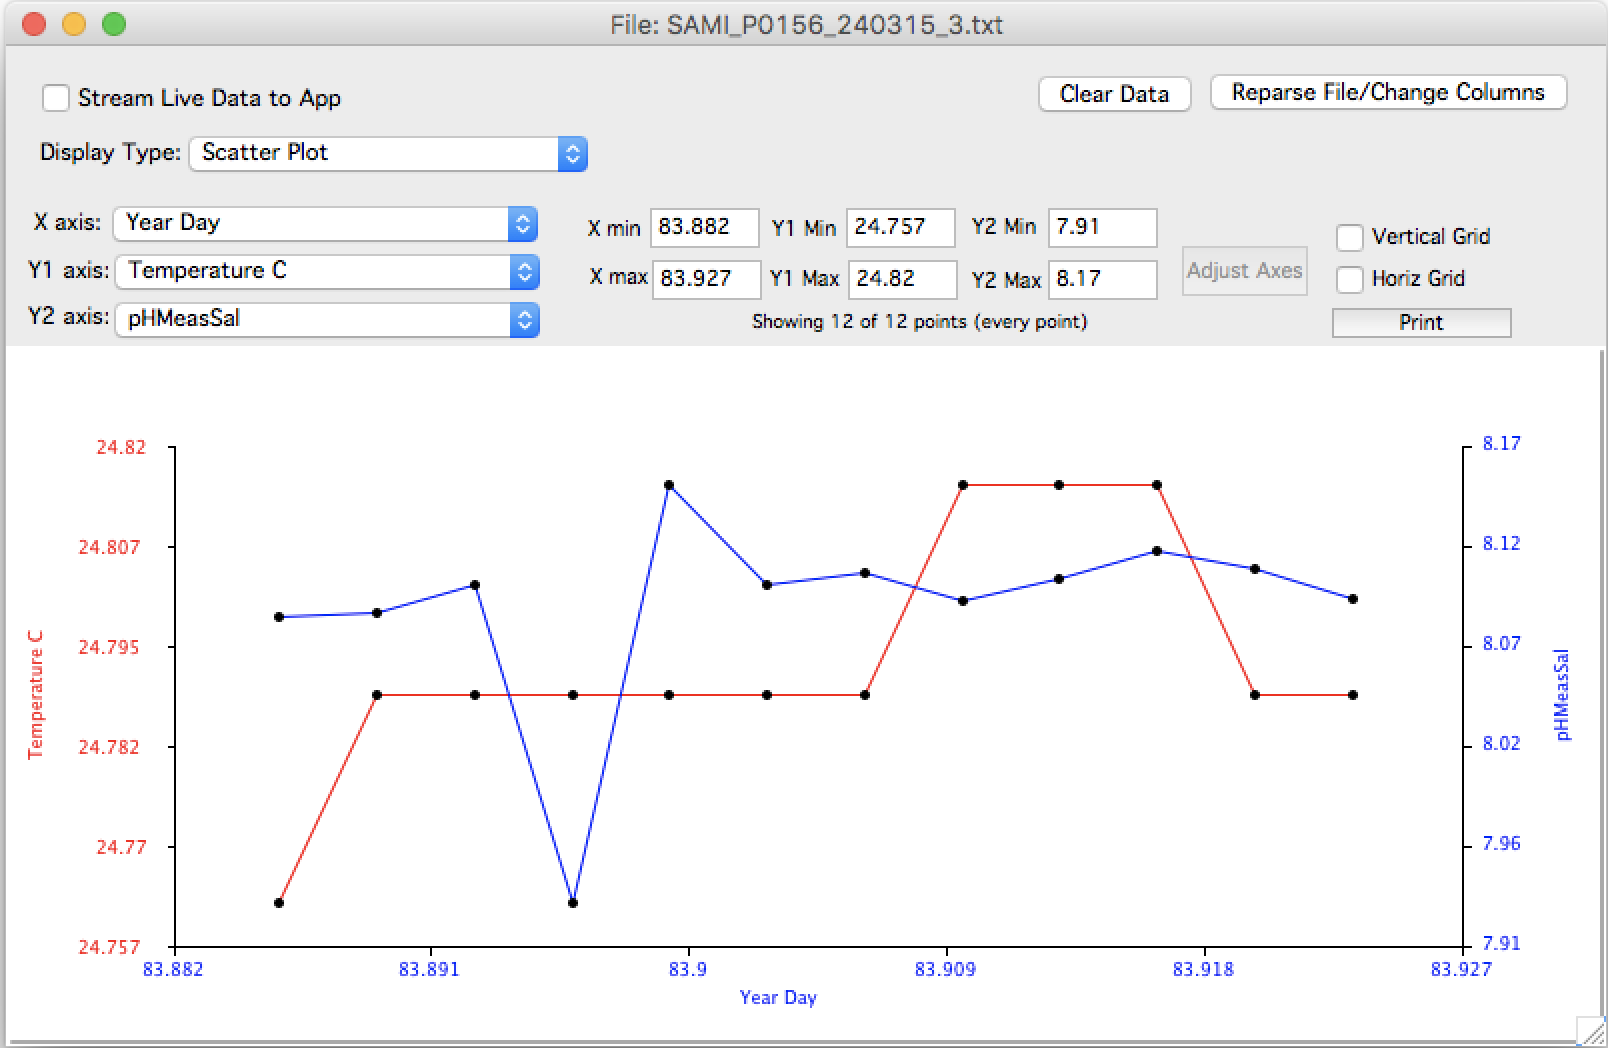
\includegraphics[width=0.7\textwidth]{figs/Plot_Data.png}
    \caption{Processed data in scatter plot format.}
    \label{fig:PlotData}
    \end{figure}
    
    \item[] \textbf{Creating your own set of parameters to view:}
    If a pre-fabricated set of parameters does not include the information that you would like to view, you may create and name your customized Column Set List. By selecting \textbf{Edit List...} from the Column Set drop-down window you will receive a Set List Editor. You may adapt a previously existing list or create a new one. 
    
    Editing a pre-existing list is done by highlighting the list you wish to edit and clicking the button in the lower right hand corner labeled \textbf{Edit}. A list of the parameters appears in a new window. The left side window labeled Columns will display all parameters contained in the Column Set List. Clicking the \textbf{Add} button below the window will make available two drop down menus on the right side of the window. The \textbf{Column Type} drop-down menu will provide you with the classifications of parameter we have to choose from. You may be interested in viewing raw data or processed data. By selecting the type of data you can choose the exact parameter you wish to plot in the Column Name drop-down menu below. There you may select from a number of different parameters to populate your Column Set List: sample or reference signals of a specific wavelength, ratio of signals to reference, temperature, time, battery voltage, and pH. 
    
    To create your own Column Set List, return to the Column Set List editor. Select \textbf{Add} from the buttons at the bottom of the window. A Column Editor will appear with an untitled Column Set List. Name your Set List and populate the parameters in the same fashion as described above.  
\end{itemize}


\subsection{Data Processing}

\subsubsection{Processing text files}

\ifcase \inst	%iSAMI

Once data has been downloaded, you can view raw and processed data with \instType{} Client software. Go to File menu and select \textbf{Open Data File}. A window will appear that asks you to select what data you want to extract from the file. In the drop down menu, select \textbf{pH\_ConstSal} for constant salinity (the approximate salinity of your sample must be entered in the \textbf{Salinity Default} box on the \textbf{Settings} tab). If you independently measured CTD data and want to use the measured salinity to calculated the pH, you will need to process the data using QC\_PH, as described in section \ref{sec:RunQC_PH}.

\or			%SAMI

Once data has been downloaded, you can view raw and processed data with \instType{} Client software. Go to File menu and select \textbf{Open Data File}. A window will appear that asks you to select what data you want to extract from the file. In the drop down menu, select \textbf{pH\_ConstSal} for constant salinity (the approximate salinity of your sample must be entered in the \textbf{Salinity Default} box on the \textbf{Settings} tab).  If you logged CTD data with the \instType{}, select \textbf{pH\_MeasSal}. If you logged CTD data independently and want to use the measured salinity, you will need to process the data using QC\_PH, as described in section \ref{sec:RunQC_PH}.

\or			%AFT

Once data has been downloaded, you can view raw and processed data with \instType{} Client software. Go to File menu and select \textbf{Open Data File}. A window will appear that asks you to select what data you want to extract from the file. In the drop down menu, select \textbf{pH\_ConstSal} for constant salinity (the approximate salinity of your sample must be entered in the \textbf{Salinity Default} box on the \textbf{Settings} tab).  If you logged TSG data with the \instType{}, select \textbf{pH\_MeasSal}. If you logged TSG data independently and want to use the measured salinity, you will need to process the data using QC\_PH, as described in section \ref{sec:RunQC_PH}.

\fi

Next, click on the \textbf{Parse File} button. Data can be viewed as a spreadsheet or Scatter Plot and exported as a text file. Although you can only view the first 500 rows of data, you can process and export the entire data file. Note that this is preliminary data.  A standalone Matlab program, included on your disc, filters and processes the data more thoroughly.  This is described in section \ref{sec:QC_PH}.


\subsubsection{Processing hex files from a custom interface}

The \instType{} data can be collected from the user's system via RS-232.  Data collected this way will be in hex format.  A hex file can be imported and processed in SAMI\_Client. From the \textbf{File} menu select \textbf{Import hex File.}  In the dropdown menu choose \textbf{pH\_const sal}. In the upper right hand corner of the Import menu, select \textbf{Choose Config File} and choose a configuration file.  A configuration file is saved when you launch the \instType{}. A generic configuration file can be saved at any time.  Once the hex data is imported, the functions of the program are the same as when reading \instType{} txt files.
\cleardoublepage\thispagestyle{empty}
\section{Processing Data With QC\_PH}
\label{sec:QC_PH}

QC\_PH is a standalone Matlab program that reads data files from the \instType{} Client. This program does a better job of filtering out outlying blanks and sample points that resulted from air bubbles, and flags those points as well as points where a mechanical error such as a failed valve or pump might have occurred. pH values calculated from SAMI\_Client and QC\_PH will differ slightly, due to blank filtering an smoothing by QC\_PH.  QC\_PH provides more reliable pH values.

\subsection{Installing Matlab Runtime and QC\_PH Application}

On the \instType{} disk, open the folder \textbf{QC\_PH}, open the appropriate folder for Macintosh or PC, then double-click on the application.  This will guide you through installation of Matlab runtime as well as QC\_PH.  It will require web access and will take a bit of time, depending on the speed of the internet connection.  Future updates to QC\_PH will install quickly, once the runtime has been installed.  If you need a complete installer (no internet access), please contact technical support. The default folder for the application is Programs\textbackslash Sunburst Sensors\textbackslash. You can move an alias of the application to a more convenient location.  

\subsection{Running QC\_PH}
\label{sec:RunQC_PH}

\begin{wrapfigure}[18]{l}{0.6\textwidth}
\centering
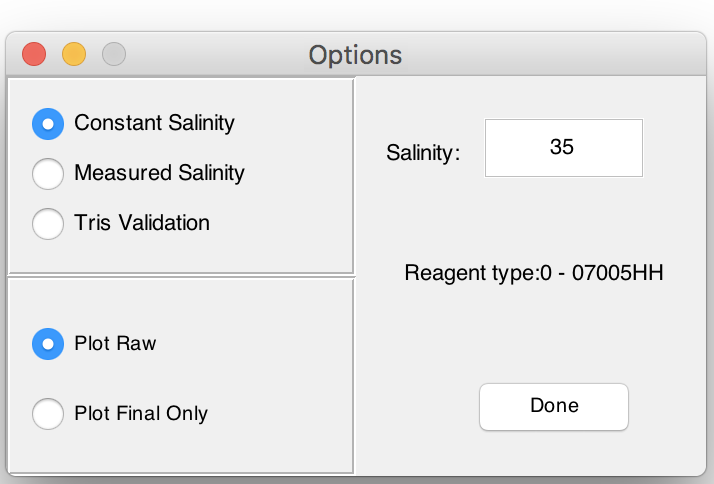
\includegraphics[width=0.9\textwidth]{figs/PH_Options.png}
\caption{PH Options.}
\label{fig:Options}
\end{wrapfigure}

To run QC\_PH, double click on the icon. You will be prompted to choose the \instType{} data file.  After reading the file, the app will ask you to choose \textbf{Constant Salinity}, \textbf{Measured Salinity}, or \textbf{Tris Validation}.  Choose \textbf{Constant Salinity} if salinity was not measured, but you know the approximate value.  Choose \textbf{Measured Salinity} if you have a data file from a CTD that was deployed with the \instType{} you will next be prompted to choose the CTD file.  This file must be a tab delimited text file in the format: dd/mm/yy Tab \normalfont {hh}$\colon$\normalfont {mm}$\colon$\normalfont {ss} Tab salinity.  Choose \textbf{Tris Validation} if you are running a Tris buffer with known pH for validation of instrument accuracy.

\begin{wrapfigure}[12]{r}{0.6\textwidth}
\centering
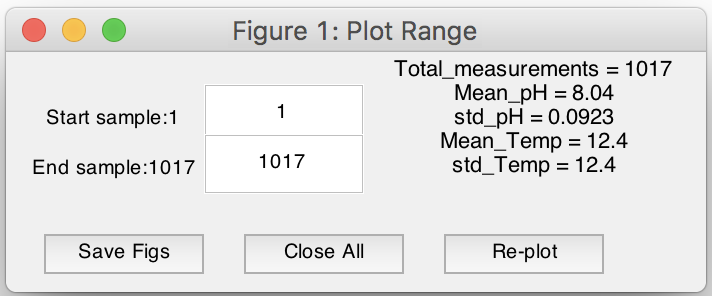
\includegraphics[width=0.9\textwidth]{figs/Plot_Range.png}
\caption{PH Options.}
\label{fig:Options}
\end{wrapfigure}

QC\_PH will calculate pH and shows plots of signals, absorbances, blanks, point pH, temperature, and final pH.  These plots can be useful in troubleshooting a \instType{}.  You can set the range of samples to view by changing the \textbf{Start Sample} and \textbf{End Sample} and selecting \textbf{Re-Plot} on Figure 1. Select \textbf{Save Figs} to save the figures and \textbf{Close All} to close the Figure windows.  Figures and a text file of the output data will be saved in a folder named \say{Filename\_Results.}

\subsection{Interpreting QC\_PH Data and Figures}
QC\_PH will plot several figures.  The figures that are often used to determine data quality and instrument performance are described here.  

The \textbf{Intensity/Absorbance} plot indicates instrument performance (Figure \ref{fig:Blanks}).  The top plot is reference signals, which should remain constant, but might degrade gradually over the course of a deployment.  The middle plot is signals through the optical cell.  These signals start high at the beginning of a sample, drop as indicator moves through the cell, and gradually increase.  Smooth curves indicate the \instType{} is working well, whereas flat lines or many spikes in signals indicates malfunction. The signals are plotted \say{Raw} and after outlying points are filtered out.

The \textbf{Blank} plot plots the signals of the blanks measured at the beginning of each sample (Figure \ref{fig:Blanks}).  These signals will degrade gradually over the course of a deployment, but should not have large spikes, and should remain above \ifcase \inst {7000.} \else {1000.} \fi

\begin{figure}[!h]
\begin{minipage}[t]{0.45\textwidth}
\centering
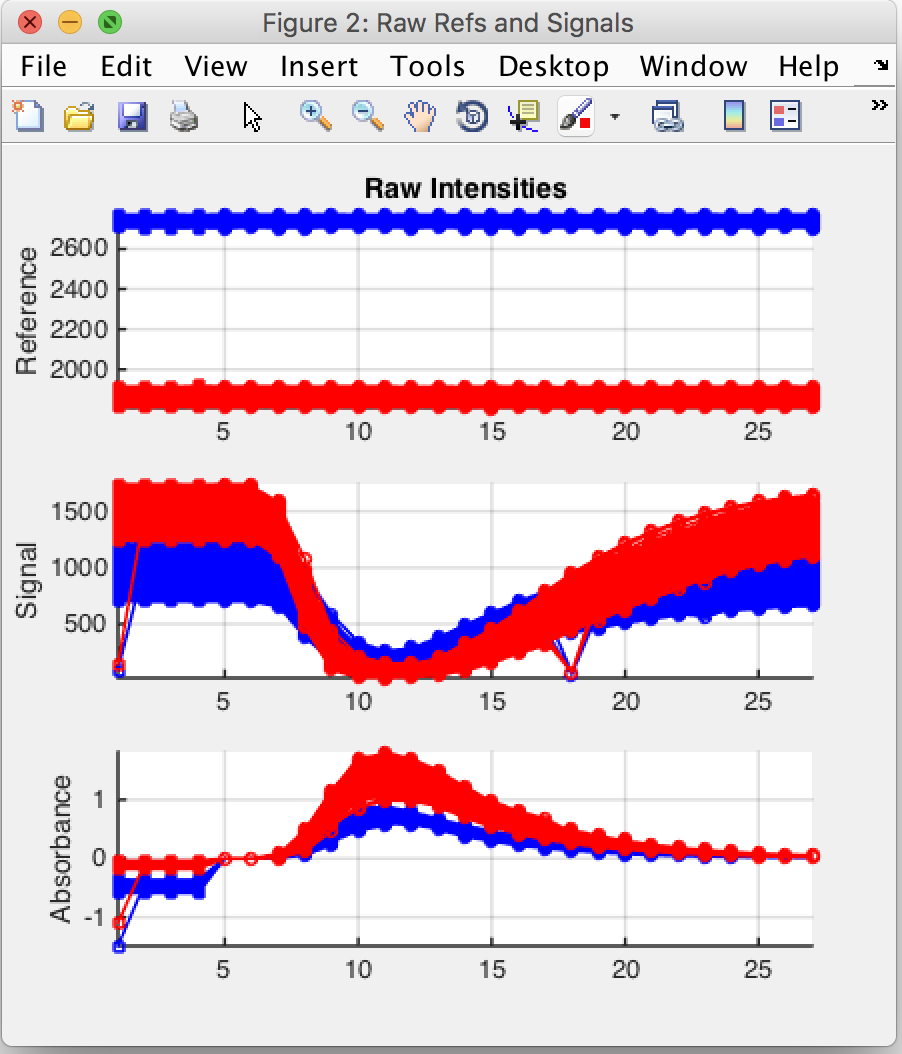
\includegraphics[width=0.9\textwidth]{figs/Intensities.png}
\end{minipage}

\begin{minipage}[t]{0.45\textwidth}
\centering
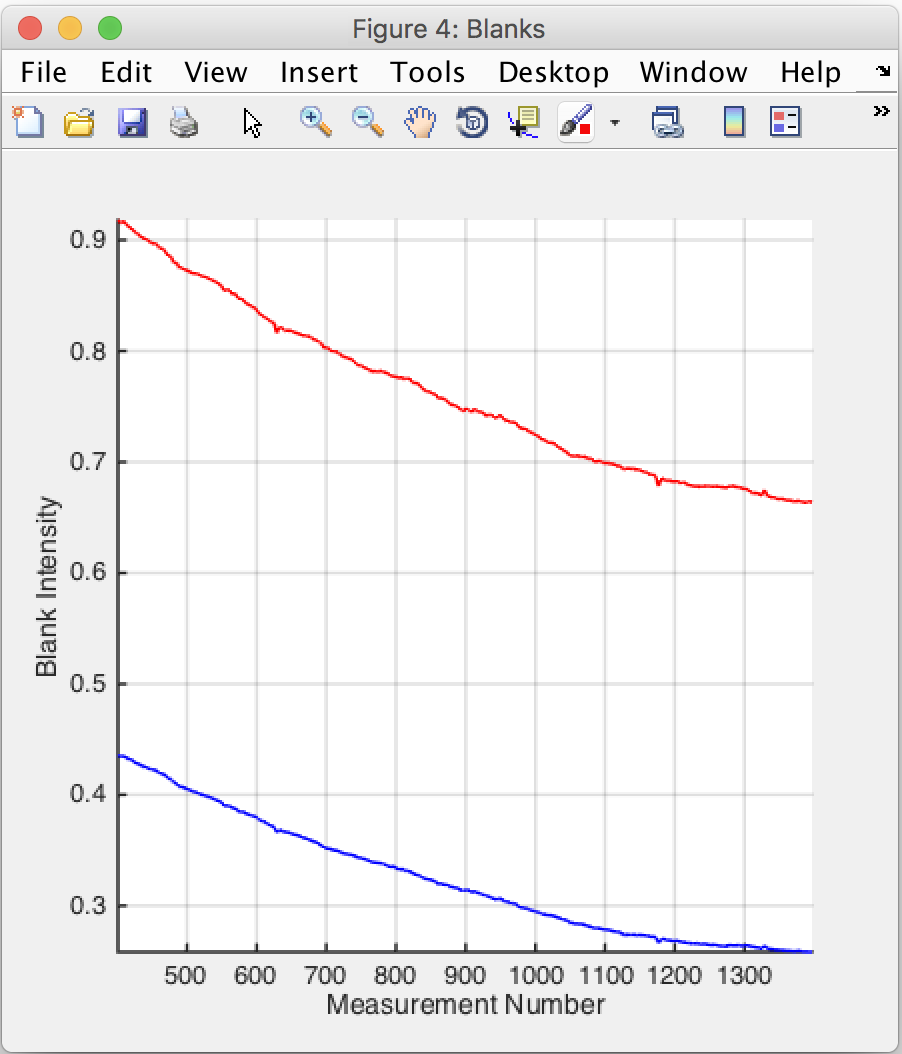
\includegraphics[width=0.9\textwidth]{figs/Blanks.png}
\end{minipage}

\captionof{figure}{Signal intensity plots (left) are plotted as 28 points for each measurement (top: reference signals, middle: signals through cell, bottom: absorbances through cell); ratios of blank signal/reference signal (right) are plotted as one point per measurement. 434\,nm signal shown in blue; 578\,nm signal shown in red.}
\label{fig:Blanks}
\end{figure}

The \textbf{Final pH} plot shows the temperature and pH measured throughout the deployment (Figure \ref{fig:FinalpH}).  pH noise from one measurement to another should be less than 0.002\,pH and temperature noise should be less than 0.05\,$\degree$C.  As blank signals degrade, pH precision might also degrade.

\begin{figure}
\centering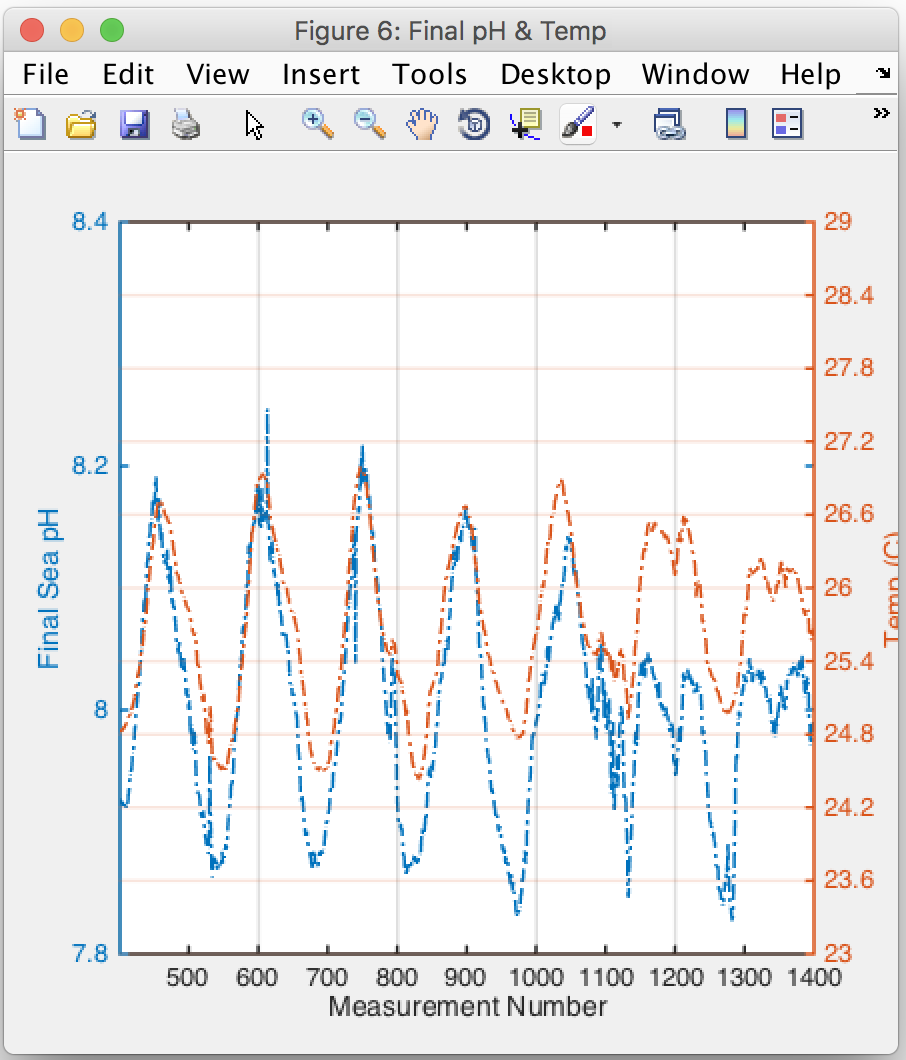
\includegraphics[width=0.6\textwidth]{figs/Final_PH.png}
\caption{Final pH (blue) and Temperatue (orange).}
\label{fig:FinalpH}
\end{figure}
\cleardoublepage\thispagestyle{empty}
\section{Care and Maintenance}


\subsection{General Cleaning}

After your \instType{} has been in use, even for short periods of time, we recommend flushing your instrument with deionized water to solvate any crystals of indicator or salt that may have formed.
{\color{red} WARNING: Failure to flush your \instType{} may result in your instrument's inability to function properly!}

Please clean the exterior of your instrument with soap and water as well as removing any sea life and plants that have made their home on your \instType{}. All other care and subsequent refurbishment should be conducted by Sunburst Sensors unless previously advised by a Sunburst representative.


\subsection{Clearing air-locked or clogged \instType{}-pH}
\label{sec:AirLock}

An air lock can occur when the instrument runs samples out of the water allowing air to be pumped into the \instType{}. If you are testing the \instType{} on a bench top, be sure to attach a bag of deionized water to the inlet or place the inlet into a beaker of deionized water. When deployed in water with high amounts of sediments, materials can also cause a clog in the instrument.  This can be cleared with the steps below.

\begin{enumerate}

    \item Fill the syringe with deionized water and connect to the intake tubing on the \instType{} (the tube protruding from the reagent chamber) as shown in Figure \ref{fig:SyringeFlush}.
    
    \begin{figure}[hb!]
    \centering
    \includegraphics[height=0.3\textheight]{figs/Syringe_\instType_Flush.png}
    \caption{Using syringe to clear air lock.}
    \label{fig:SyringeFlush}
    \end{figure}
    
    \item Connect the \instType{} to a computer with the client software installed; connect to the instrument and start the software. In the \textbf{Utility} tab under the \textbf{Cycle Pump} panel, set the \textbf{\# cycles} to 10. Apply a constant pressure to the syringe and click \textbf{Run}.  \textbf{Open Valve} should \textit{NOT} be checked.
    
    The deionized water should move through the system and come out of the cell outlet tube (top of \instType{}). This step may be repeated a couple of times. If the water does not move through the instrument, contact Sunburst Sensors for additional technical support. 
    
    \item Once fluid begins to move through the system, insert the intake tubing (the tube with the blue fitting where the syringe was attached) into a beaker with a few hundred milliliters of deionized water, or connect the blank bag to the inlet. 
    
    \item Next flush the \instType{} using deionized water from the beaker or the bag. On the Utility tab under the \textbf{Cycle Pump} panel set the \# of cycles to 99 and click on \textbf{Run}. Make sure the intake tube is in the deionized water before pressing the \textbf{Run} button.  \textbf{Open Valve} should \textit{NOT} be checked.
    
    The deionized water should move through the system normally. If the water is not moving through the instrument, contact Sunburst Sensors for technical support at techsupport@sunburstsensors.com.
    
    \item Once water runs through the instrument, reconnect the tubing to the mixer. 
    
    \item Insert the intake tubing (the tube with the blue fitting where the syringe was attached) into a beaker with a few hundred milliliters of deionized water or connect the blank bag to the inlet. 
    
    \item Next flush the \instType{} using deionized water from the beaker or bag. On the Utility tab under the \textbf{Cycle Pump} panel set the \# of cycles to 99 and click on \textbf{Run}. Make sure the intake tube is in the deionized water before pressing the \textbf{Run} button.  \textbf{Open Valve} should \textit{NOT} be checked.
    
    If the water is not moving through the instrument, contact Sunburst Sensors for additional technical support.
   
\ifcase \inst	%iSAMI

    % Don't say anything about brass cage.

\or			%SAMI

    \item If the \instType{} is functioning correctly, re-attach the brass cage using zip ties. Trim off the remaining tails of the zip ties.

\or			%AFT

    % Don't say anything about brass cage.
    
\fi

\end{enumerate}

\clearpage


\section{Troubleshooting}

These are a few common questions that we receive at Sunburst Sensors. If you do not see your question here, please contact us at techsupport@sunburstsensors.com. 

\paragraph{\underline{What do I do if I cannot communicate with the instrument?}}
You will not be able to communicate with your instrument if the correct serial port has not been selected. In SAMI\_Client select \textbf{Edit $\rightarrow$ Preferences} and try choosing another serial port from the menu. Many times it may take some time for the computer to fully populate the list. You may need to wait until another serial port appears in the drop-down menu.  The COM port on the PC will typically be the last one in the list. On a Mac the serial port will be named \verb|USB-serial XXXXXXXX| where ``X'' represents alpha-numeric characters.

On Windows operating systems (XP, Vista, 7, 10) it is sometimes helpful to go to the Device Manager (Control Panels, System and Maintenance, System) and look for the Ports to verify your USB-Serial converter is working.  There should be at least one USB Serial Port under \textbf{Ports (COM \& LPT)}. Double click to open and verify that it is the FTDI converter and not some other device.  Use this port number in the SAMI Client Preferences.

If you do not see a USB serial port, it is likely that you will need to install the driver. Try unplugging and re-plugging the cable to the PC. This should prompt an install dialog. The driver is on the install CD and can also be found here: \url{http://ftdichip.com/Drivers/VCP.htm}

On some PCs switching to another USB port will solve the problem. Also, it is occasionally useful to restart the \instType{} Client software and/or the PC itself.

\paragraph{\underline{What happens if the signals drop?}}
This is very likely due to an obstruction in the path of the optical cell. Commonly, it is air bubbles which can be flushed out by continually pumping. If you use the \textbf{Cycle Pump} function on the Utility Tab of SAMI\_Client to pump deionized water (after attaching DI bag to inlet) through the instrument the problem will often be resolved.

\paragraph{\underline{What should the signal intensities be?}}

\ifcase \inst	%iSAMI

Signal intensities can range from 0 to 16383. If any signal intensity is at or near 16000, the channel may be saturated with light, giving erroneous results. Reference and signal intensities should be greater than $\sim$\,6000 for a blank (DI, seawater, etc.).  Lower intensities will result in higher noise in absorbance and thus pH measurements. However, if during a measurement signal intensities are low but reference intensities are not, the flow cell needs to be flushed. Dark signals will normally range from $\sim$\,200--400. Higher or erratic dark signals could indicate an electronic problem with your \instType{}.  Contact Sunburst if any abnormal signals cannot be rectified.

\else			%SAMI/AFT

Signal intensities can range from 0 to 4905. If any signal intensity is at or near 4800, the channel may be saturated with light, giving erroneous results. Reference and signal intensities should be greater than $\sim$\,2000 for a blank (DI, seawater, etc.).  Lower intensities will result in higher noise in absorbance and thus pH measurements. However, if during a measurement signal intensities are low but reference intensities are not, the flow cell needs to be flushed. Dark signals will normally range from $\sim$\,100--200. Higher or erratic dark signals could indicate an electronic problem with your \instType{}.  Contact Sunburst if any abnormal signals cannot be rectified.

\fi

\paragraph{\underline{How do I flush my \instType{}?}}
There is a function on the Utility Tab of the \instType{} Client labeled \textbf{Cycle Pump}. Under cycle pump you may flush your \instType{} without disrupting the programmed measurement routine.  In addition, the user may use the de-clogging kit that is included with all new pH instruments.  See the next chapter for instructions on using the de-clogging kit.

\paragraph{\underline{My Spreadsheet Maker did not populate the Column Set List!}}
It is very likely that the file included on your instrument disc was not copied over to your computer. Please double check that every file on the disc has been successfully transferred including a file labeled \verb|ColumnSettings.txt|.   

\paragraph{\underline{What if I cannot rectify my problem?}}
Contact Sunburst Sensors, our information is found on the front of this manual. We will work with you to find the fastest and most economical solution to your problem. Never hesitate to give us a call or send us an e-mail at techsupport@sunburstsensors.com.
\cleardoublepage\thispagestyle{empty}
% Use \cmdfont{} macro to change font to courier for indicating command literals.

\section{Low level operation of the \instType{}}

The \instType{} has a very robust, user-friendly client that is recommended
for programming, downloading, and updating. That being said, there are
some users who wish to be able to have a lower level control of the
instrument. This document attempts to explain the low level operation of
the \instType{}.


\subsection*{RS-232 Serial Communication}

The \instType{} uses RS-232 to communicate with 8-none-1 settings. RTS must
be held high to turn on the RS-232. When RTS is asserted the \instType{}
will begin to send status strings every second. For interactive use,
these status strings should be turned off using the \cmdfont{F5A} command (see
Low Level Commands below). Once this command is issued, however, the
client software will not recognize the \instType{} as being connected. It can
be turned back on by \cmdfont{F01} if you need to use the client.

Once communications have been established the \instType{} needs to be
stopped, if it is running, downloaded, if there is data and erased.

The command sequence for this is:
\begin{quote}
	\cmdfont{\textbf{Q5A}} - stop running and close memory\\
	\cmdfont{\textbf{D\#\#}} - send \#\# pages of memory over serial port\\
	\cmdfont{\textbf{E5A}} - erase memory, including RAM variables
\end{quote}

At this point the \instType{} must be configured before it can be used
again, setting the time, sample interval, etc. Configuration is
discussed in section below. While the \instType{} do not have a strict
polling mode, they can be configured to start long in the future and
sent commands to do measurements in the interval. To get a measurement,
once the unit is configured, just send \cmdfont{R}. (All commands are \cmdfont{CR}
terminated as discussed below.)

\subsection*{Configuring the \instType{}}

The configuration string sets the various parameters required by the
\instType{} to operate. It sets the time and date, the start time and end time.
It tells the \instType{} which drivers to use for the \instType{} itself (e.g. is it a
pH unit or \dioxide{} unit?) and what drivers to use for any devices that are
connected to the \instType{}. The configuration string also contains all the
parameters required by the various drivers, including timings of pumps,
valves, etcetera.

The configuration string is 116 bytes (232 hex characters) in length,
which is padded to 128 bytes (256 hex characters), followed by 128 bytes
(256 hex characters) of user text and terminated with a null
character. Each byte is represented by a two character hex string. The
beginning of the string specifies the time parameters and mode, followed
by sampling intervals, driver info and pointers to parameters.

The configuration string is sent or retrieved to/from the \instType{} by client
software using \cmdfont{L} command which is described on page \pageref{sec:Lcommand}.\\
\begin{center}
\colorbox{lightgray}{+++++++\textbf{Overview of Configuration String for Firmware 50+}++++++++}\\
\end{center}


\begin{tabular}{ m{10em} m{12em} m{2em} <{\centering} m{8em} <{\centering} } 

\textbf{Description} & \textbf{Units} & \textbf{bytes} & \textbf{position in string} \\
Launch time (GMT) 		& secs from 1/1/1904 	& 4 	& 0 \\
Start time from launch 	& secs from launch 		& 4 	& 8 \\
Stop time from start 		& secs from start 		& 4 	& 16 \\
Mode 				& switch bits (see below) 	& 1 	& 24 \\
 & & & \\
 \multicolumn{4}{l}{\underline{For \instType{}, Dev1, Dev2, Dev3, Prestart} \underline{(5 per row)}}\\
Interval 			& secs 			& 3 	& 26, 36, 46, 56, 66\\
Driver 			& n/a 			& 1 	& 32, 42, 52, 62, 72\\
PointerToParams 	& offset from pos 78	& 1 	& 34, 44, 54, 64, 74\\
 & & & \\
Global configuration & switches 		& 1 	& 76\\
\end{tabular}

\begin{quote}
	Bit 0 Run main serial port at 57600 or 9600\newline
	Bit 1 Send \^{}(record type) before a driver starts\newline
	Bit 2 Send live records over serial\newline
	Bit 3..6 Not assigned, set to zero\newline
	Bit 7 Extend Global config.\newline
\end{quote}

\underline{For \instType{}, Dev1, Dev2, Dev3, Prestart} \underline{(pointed to by above)}

Parameter bytes        various       max of 15       78 for \instType{}, others vary

Max config string length = 13 + (5x5) + 1 + (5x15) = 114 bytes (228 hex
chars, padded to 256 chars)

\textbf{Mode bits}

\begin{quote}
	Bit 0 PMI sampling schedule enabled\newline
	Bit 1 \instType{} sampling schedule enabled\newline
	Bit 2 Slot 1 follows \instType{} sample\newline
	Bit 3 Slot 1 independent schedule\newline
	Bit 4 Slot 2 follows \instType{} sample\newline
	Bit 5 Slot 2 independent schedule\newline
	Bit 6 Slot 3 follows \instType{} sample\newline
	Bit 7 Slot 3 independent schedule\newline
\end{quote}

\begin{center}
\colorbox{lightgray}{++++++++++++++++++++++++++++++++++++++++++++++++++++++}\\
\end{center}


\subsection*{Example of a Configuration String}

SAMI-\dioxide{} programmed on Oct. 6, 2011

\instType{} uses driver 4,5 (\dioxide{}-average) on 30 min intervals

All devices follow \instType{}

Device 1 - Serial +\,Power\newline
Device 2 - Generic 0--5\,V +\,Power\newline
Device 3 - Power\newline
Prestart - 4 hour intervals for DI pump\newline

\clearpage

:ConfigHex (232 characters)

\colorbox{green}{CAB39E84}\colorbox{red}{000000F4}\colorbox{lightgray}{01E13380}57\colorbox{yellow}{000708}04010\colorbox{violet}{00258}030A\colorbox{orange}{000258}0017\colorbox{green}{000258}011A\colorbox{lightgray}{003840}001\newline C\colorbox{yellow}{07}\textcolor{blue}{1020FFA8181C010038}\textcolor{red}{10010120256400043338333500}\textcolor{green}{020001}0200000000000000000000000\newline 000000000000000000000000000000000000000000000000000000000000000000000000000000000


\subsection*{General timing and mode}

\begin{itemize}
\item[]
\colorbox{green}{CAB39E84} - \underline{Time of programming (GMT) - Oct 6, 2011 18:05:56 (total seconds from 1/1/1904)}\\
\colorbox{red}{000000F4} - \underline{Time until start - 244 sec}\\
\colorbox{lightgray}{01E13380} - \underline{Time from start until stop - 365 days (315360000 sec)}\\
57 - \underline{Mode bits - (01010111 - Bits 6,4,2 = all devices follow \instType{}
sample, bit 0= prestart schedule on,} \linebreak \underline{bit 1 = \instType{} schedule on)}\\

\item[]
\colorbox{yellow}{000708} - \underline{\instType{} interval (1800 sec - 30 min)}\\
04 - \underline{\instType{} Driver (\dioxide{} Ave+)}\\
01 - \underline{Pointer to params (\instType{} always 01)}\\

\item[]
\colorbox{violet}{00258} - \underline{Device 1 interval (10 minutes - overridden by mode bits
above)}\\
03 - \underline{Device Driver}\\
0A - \underline{Pointer to params} \underline{(position relative to byte 1 of \instType{}
driver in bytes)}\\

\item[]
\colorbox{orange}{00258} - \underline{Device 2 interval (10 minutes - overridden by mode bits
above) }\\
00 - \underline{Device Driver}\\
17 - \underline{Pointer to params (position relative to byte 1 of \instType{} driver
in bytes)}\\

\item[]
\colorbox{green}{000258} - \underline{Device 3 interval (10 minutes - overridden by mode bits
above) }\\
01 - \underline{Device Driver}\\
1A - \underline{Pointer to params (position relative to byte 1 of \instType{} driver
in bytes) }\\

\item[]
\colorbox{lightgray}{003840} - \underline{Prestart interval (14400 sec - 4 hours)}\\
00 - \underline{Driver}\\
1C - \underline{Pointer (pre-start has no params)}\\
07 - \underline{Global parameter switch - send live records, with record type
early at 57.6K}
\end{itemize}


\subsection*{Parameters pointed to}

\begin{itemize}
\item[]
\textcolor{blue}{1020FFA8181C010038} - \underline{driver 4 parameters (SAMI-\dioxide{} Average+
driver) see below}

\item[]
\textcolor{red}{10010120256400043338333500} - \underline{parameters for serial + power driver}

\item[]
\textcolor{green}{020001} - \underline{02 Duration 00 Power select 01 \# samples to average}

\item[]
0200 - \underline{02 Duration 00 Power select}

\item[]
Padding\\
000000000000000000000000000000000000000000000000000000000 \linebreak 0000000000000000000000000000000000000000000
\end{itemize}


\subsection*{SAMI-CO$_\mathrm{\textbf{2}}$ Driver 4/5 Parameters explained}

In the example above the SAMI-\dioxide{} is using driver 4/5, which is default.
The parameter string 1020FFA8181C010038 is sent. The meaning of this
string is shown in figure and table below.


\subsection*{Low Level Commands}

The \instType{} client software utilizes a relatively simple
vocabulary of comands to interact with the \instType{}.

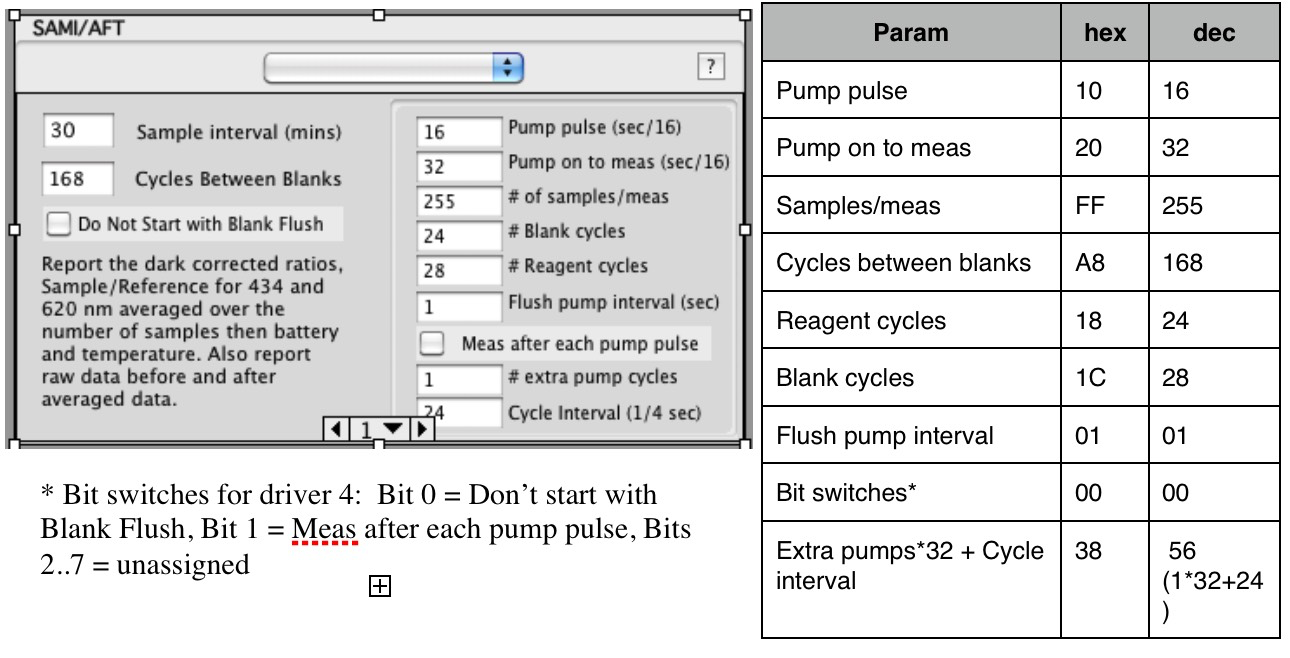
\includegraphics[width=\textwidth]{figs/Image1.png}


\subsection*{Command Format}

\begin{itemize}
\item
  Command format: one letter followed by a number of arguments as hex
  numbers and ending with carriage return (\cmdfont{CR}).
\item
  Args may be separated by Space, Tab, comma, '/' or ':' the first
  separator may be omitted. For example "T 03/05/29 5 12:30:06" is
  equivalent to "T3 5 29,5,12 30 06"
\item
  123 is equivalent to 000123 if a long word is expected 0123 if a word
  or 23 if a byte.
\item
  If more bytes are entered than the command uses the left most (first
  entered) bytes are ignored. For example, a command that takes a byte
  will read \cmdfont{1A2B} as \cmdfont{2B}.
\item
  Arguments are represented as follows:
\end{itemize}

\begin{quote}
(\cmdfont{B}) One byte (\cmdfont{S}) 12 bits (\cmdfont{W}) 2 bytes (\cmdfont{L}) 3 bytes (\cmdfont{E}) 4 bytes (\cmdfont{X}) don't
care, () none, (\cmdfont{N}) nibble

\{\} indicates return expected using above while \{R\} means returns
record

(\cmdfont{5A}) sending \cmdfont{5A} enables a variant of the commands normal function
\end{quote}

\begin{itemize}
\item
  Arguments in {[} {]} are optional. Typically these optional arguments
  are present for a ``write'' to the \instType{} and omitted if the user wants
  to ``read'' from the \instType{}.

\item
  No backspace or delete support for cmds sent - type non-hex arg with
  \cmdfont{CR} to abort.

\item
  Results (reads) are returned as space separated hex and terminated
  with \cmdfont{CR}.

\item
  Commands that are illegal or malformed return \cmdfont{?}, error code in hex
  followed by return.

\item
  Any input returns \cmdfont{!} if a command or process is running.

\item
  Echo is off by default. Echo off suppresses prompts and error text.
  Use \cmdfont{I} command to enable echo.
\end{itemize}


\subsubsection*{Command List}

%C run blank
{\cmdfont{\textbf{C}} ()\{R\} Run Blank cycle on SAMI-\dioxide{}}
\begin{quote}
	() - no argument required\\
	\{R\} - returns a data record\\
	A valid configuration is required. If \instType{} erased then error returned.\\
	Returns (and if running writes) a data record.\\
\end{quote}

%D dump memory
{\cmdfont{\textbf{D}} (W,{[}B{]},{[}W{]}) \{memory stream\} Dump Memory}
\begin{quote}
	(W - arg1) is number of pages beginning from page 0.\\
	{[}B - arg2 {]} - optional format switch 0 for binary, 1 for hex
	(default is binary)\\
	{[}W - arg3 {]} - optional start page\\
	B - bit 0=1 send as hex return after page, bit 0=0 send as binary\\
	Begins streaming memory with first data record.\\
\end{quote}

%E erase
{\cmdfont{\textbf{E}} ({[}B{]})\{W\} Erase}
\begin{quote}
	() - no argument erases \instType{} memory\\
	(5A) - for safety erase all of memory and clear ram vars.\\
	\{W\} - returns the first unerased page or 8000 if all are erased\\
	Erase shuts down all activity including time keeping but allows serial
	commands.\\
	Stops real time clock\\
\end{quote}

%F status ticks
{\cmdfont{\textbf{F}} (B)() Status ticks on/off \& special cmd mode}
\begin{quote}
	(5A) - turns ticks off -turn off 1/sec status from \instType{} Enable Debug
	commands\\
	(55) - turns on optional commands (see section below)\\
	(any other byte) - turns ticks on and disables optional commands\\
\end{quote}

%G open flash
{\cmdfont{\textbf{G}} ({[}B{]})() Open flash and start recording}
\begin{quote}
	Starts real time clock if it is not running
	Clears n\_drec number of records, n\_erec number of error records.
	n-bytes Number of bytes stored - Is set to the start of the page after
	the last un-erased page.
	Restarting without erase is supported.\\
\end{quote}

%H read ADC channel
{\cmdfont{\textbf{H}} (N)\{S\} Read one adc channel}
\begin{quote}
	(N) - Channel 0..7 or\\
	\{S\} - returns in Hex ADC count Voltage = (S/4096)*5.00V\\
	0 - Photo Reference, gated in firmware so not useful\\
	1 - Photo Signal, gated in firmware so not useful\\
	2 - Battery if 12V is enabled else 0 V= count/4096*5V*3 Volts\\
	3 - Thermistor\\
	4 - 3rd Party input J6 pin8 - 5V full scale\\
	5 - 3rd Party input J6 pin8 - 5V full scale\\
	6 - 3rd Party input J6 pin8 - 5V full scale\\
	7 - 3rd Party input J6 pin8 - Photo diode amplified current input\\
	
	\underline{Special}
	
	If arg $\geq$\,80 turn on 12\,V and read Batt, therm, 5\,V in 1, 5\,V
	in 2, 5\,V in 3, photodiode restore 12\,V
	
	Returns \{S S S S S S\}\\
\end{quote}

%I immediate read
{\cmdfont{\textbf{I}} ({[}B{]})\{B\} Immediate read status sw \& bus}
\begin{quote}
	arg switches\\
	Bit 0 Pump on\\
	Bit 1 Valve on\\
	Bit 2 12V on\\
	Bit 3 Reserved - was Battery sense enable\\
	Bit 4 debug LED off\\
	Bit 5 echo off\\
	Bit 6 Reserved\\
	Bit 7 Reserved\\
	Return Switches \{B\} as in arg\\
\end{quote}

%J invoke loader
{\cmdfont{\textbf{J}} (B) invokes loader returns nothing, used to load firmware
after erase}
\begin{quote}
	(5A) - branch to loader\\
	(5C) - Erase Board Type and SN 128 Bytes in microcontroller flash\\
\end{quote}

%L load or read config
\label{sec:Lcommand}
{\cmdfont{\textbf{L}} ({[}5A{]})\{ConfigString\} Load or Read Config + UserText}
\begin{quote}
	-\/- Read or load a string. Consisting of Configuration string (+ fill to
	256 bytes) + UserText\\
	() No argument gets configuration string from board.\\
	(5A) - start 4 byte timer at zero and wait for \cmdfont{CR} from board
	After receiving carriage return, send load data as packed hex with no
	separator.\\
	First non-hex non-return character causes abort of load.\\
	Either a null between byte 256 and 512 or 512 bytes is a valid\\
	termination. Any non hex is an error.\\
	Returns 2-byte checksum read from flash after write.\\
	Successful load starts real time clock. Erase or reset stops clock\\
\end{quote}

%M measure LEDs 
{\cmdfont{\textbf{M}} ({[}B{]})\{S,S,S,S,S,S\} Measure LEDs w/o pumping}
\begin{quote}
	Read the ADC values no pump cycle\\
	Arg default = FF (read all)\\
	Bits enable sending of data below bit 2..7 - blue ref...dark signal\\
	Returns \{S\} in same order as below\\
	bit2 - Dark ref\\
	bit3 - Dark signal\\
	bit4 - LED1 ref\\
	bit5 - LED1 signal\\
	bit6 - LED2 ref\\
	bit7 - LED2 signal\\
\end{quote}

%N -compare
{\cmdfont{\textbf{N}} ( {[}B{]} B W W) }
\begin{quote}
	Compare or write a byte value to a range of memory W as page count\\
	Verify N(byte value, word Start\_page, word count\_pages) Return (0 if
	true, first failed page if false)\\
	Write N(\$5A, byte value, word Start\_page, word count\_pages)\\
	Progress reporting\\
	Returns hight byte of page +1 for each page started then XX last page
	address where XX=00 for good FF for fail\\
	(Should fix this, should be page started then 2 byte end address and 00
	or FF)\\
\end{quote}

%O readwrite port
{\cmdfont{\textbf{O}} ({[}B{]}) \{B\} Read or write port A - set bits enable power
out function}s
\begin{quote}
	() - no arg is `read' with \{B\} returned as described below\\
	(B) - arg writes to port A to turn on/off power out as below
	
	Bit0 - 12\,V\\
	Bit1 - Valve - J4 pin6\\
	Bit2 - Pump - J4 pin7\\
	Bit3 - 3rd party power J5 pin 6\\
	Bit4 - 3rd party power J5 pin 5\\
	Bit5 - 3rd party power J5 pin 4\\
	Bit6 - Select 12\,V for 3rd party power\\
	Bit7 - Select Battery for 3rd party power\\
	Note that if both bit 6 and 7 are set, bit 7 is cleared - 12\,V is
	selected\\
\end{quote}

%P - pump valve
{\cmdfont{\textbf{P}} ({[}B{]},{[}B{]}) Pump and valve powering}
\begin{quote}
	() - no argument pump and valve off\\
	(B1) - one arg set pump and valve on or off\\
	(B1,B2) - 2 args set on or off and restore after arg2 1/8 seconds\\
	B1 - bit 0 turns pump on, bit 1 turns valve on\\
	B2 - time to hold state of B1 before returning to original state (1/8's
	sec)\\
	Turns on 12\,V supply if required and restores to original state\\
	Return Null just carriage return after time out - single threaded\\
\end{quote}

{\textbf{Q} (5A)() Close flash and stop recording.}\\

%R run sample
{\cmdfont{\textbf{R}} ({[}B{]})(R) Run sample cycle on device}
\begin{quote}
	Arg Slot Default device is \instType{} - 0 slot1..3, PMI is 4\\
	Arg set bit 3 returns test error/info rec\\
	Arg bit 2 selects error/info record\\
	A valid configuration is required. If erased then error.\\
	Returns (and if running writes) a data record\\
\end{quote}

%S - status report
{\cmdfont{\textbf{S}} ({[}B{]})\{: E,W,L,L,L,W,W\} Ask for status from \instType{} (note
this is auto sent when RTS is high)}
\begin{quote}
	(B) If arg=0 (default) returns \cmdfont{:} followed by \cmdfont{:}\\
	\{E\} time in seconds since \cmdfont{L} command - Cleared by Erase\\
	\{W\} statusflags - Cleared by Erase, defined here:
\end{quote}

\begin{quote}
	bit 0 Clock started\\
	bit 1 Recording started\\
	bit 2 Recording ended on time\\
	bit 3 Recording ended memory full\\
	bit 4 Recording ended due to error, failure, or user stopped\\
	bit 5 Data downloded\\
	bit 6 Flash Open\\
	bit 7 *Low or no battery before start 256*t\_pmi seconds - fatal\\
	bit 8 Battery low on measure cycle - fatal\\
	bit 9 Battery low on blank cycle - fatal\\
	bit 10 *Battery low on external device cycle - fatal\\
	bit 11 *External device 1 fault - fatal for device shut it down\\
	bit 12 *External device 2 fault - fatal for device shut it down\\
	bit 13 *External device 3 fault - fatal for device shut it down\\
	bit 14 Erased\\
	bit 15 Power on flags not valid
	
	( * Not yet implemented )\\
\end{quote}

\begin{quote}
	\{L\} - n\_rec (3) number of data records - Cleared by Erase\\
	\{L\} - n\_erec (3) number of error records - Cleared by Erase\\
	\{L\} - n\_bytes (3) Number of bytes stored including config and user
	text as full pages - Cleared by Erase\\
	If arg=1 returns Name(16) SN(4) FirmwareVer(4) \instType{} board version(2)
	\instType{} board Config(2) Cal(24) Cksum(1)\\
	If arg=2 returns 128 bit microcontroller flash Name(16) SN(4)
	calibration TBD Checksum(1)
\end{quote}


\subsubsection*{Commands turned on by \cmdfont{F55} command }

\cmdfont{\textbf{@}} ({[}X{]},{[}X{]},{[}X{]}...)(T) Test the command parser
\begin{quote}
	Debug tool only works if echo is on.\\
	Reports in text the number and value of args.\\
\end{quote}

\cmdfont{\textbf{A}} (X)(T) List all commands
\begin{quote}
	Debug tool only works if echo is on.\\
	Lists all the commands.\\
\end{quote}

\cmdfont{\textbf{B}} ( )(S) Battery Voltage
\begin{quote}
	S the battery voltage 12\,V must be enabled $V_bat = Arg * 5 * 3 / 4096$\\
\end{quote}

\cmdfont{\textbf{T}} () (s) Thermistor Voltage
\begin{quote}
	$V= 4096 * Thermistor Res / (Thermistor Res + 17400)$
\end{quote}


\subsubsection*{Debug tools hidden - enabled by \cmdfont{F5A}}

\cmdfont{\textbf{Z}} (W)( ) Set breakpoint

\cmdfont{\textbf{\^{}C}} Break to debugger

\cmdfont{\textbf{\^{}T}} Show current program address and reg.


\subsubsection*{Extra debug commands for now}

\cmdfont{\textbf{K}} Send error \cmdfont{CF} with 2 extra bytes \&h0201

\cmdfont{\textbf{V}} No arg send 'Hello World' out secondary port and echo for 10 sec then
return 'Done'

\cmdfont{\textbf{V}} Any arg send 'Hello World' out serial port and return 0 if all\\
characters echo - for tester

\cmdfont{\textbf{W}} Return status word, MFG code, etc.

\cmdfont{\textbf{X}} Sleep for ever but wake every 8 sec and send time - reset to exit

\cmdfont{\textbf{Y}} Show time, internal flags, wake counter


\subsubsection*{Notes}

While DTR is present on the serial port command mode is maintained and 5\,V power is on. 12\,V power is off by default but can be turned on with \cmdfont{I} or \cmdfont{O} command.

12\,V power will cycle on and off as needed to run pump or valve.

\subsubsection*{*** Command Error Codes ***}
\begin{quote}
	\cmdfont{00} Wrong Number of Arguments\\
	\cmdfont{01} Command Not Implemented\\
	\cmdfont{02} Invalid Arguments\\
	\cmdfont{03} Command Buffer Overflow\\
	\cmdfont{04} Invalid Command Enter A return for a list of commands\\
	\cmdfont{05} Error in config data\\
	\cmdfont{06} \textgreater{} 2000 pages\\
	\cmdfont{07} Invalid Configuration\\
	\cmdfont{08} Bad Key\\
	\cmdfont{09} Flash is Open\\
	\cmdfont{0A} Flash is Not Open\\
	\cmdfont{0B} Too Many Arguments\\
	\cmdfont{0C} Too Few Arguments\\
	\cmdfont{0D} Memory Full\\
    	\cmdfont{0E} Not Valid With Echo Off\\
	\cmdfont{0F} Unimplemented Extenstion Index in Configuration\\
	\cmdfont{10} Flash Data not erased\\
	\cmdfont{11} Invalid Arguments
\end{quote}

\clearpage

\subsection*{Error conditions}

No battery - If main battery without load at wake from sleep is below
Vmin.

\instType{} counts no battery event and schedules next wake for measurement.

Note that \instType{} does not attempt to write Flash memory on backup battery.

If 2 byte no battery count overflows \instType{} shuts down completely.

If \instType{} awakes to find battery restored it writes an error record with
counts and time and resumes normal operation.

Battery fail - if \instType{} tries to power up analog, pump, valve, or
external device and battery falls below Vmin:
\begin{itemize}
	\item[]
	write an error record
	
	\item[]
	close Flash page
	
	\item[]
	shutdown completely until handshake from host.
\end{itemize}
\cleardoublepage\thispagestyle{empty}
\section*{Warranty}
\label{sec:Warranty}
\addcontentsline{toc}{section}{\nameref{sec:Warranty}}

\begin{sans}

Sunburst Sensors, LLC warrants to the original purchaser that instruments manufactured by Sunburst Sensors shall be free from defects in materials and workmanship for the life of the product. Under this warranty, the instrument will be repaired or replaced as deemed appropriate by Sunburst Sensors without charge for parts or labor when the instrument is shipped prepaid to our location. This warranty does not apply to any instrument which has not been installed or used in accordance with proper operation and installation specifications. Sunburst reserves the right to void any warranty, written or implied, if upon Sunburst's examination of the instrument reveals failure was due solely, or in part, to accident, misuse, neglect, abuse, alteration, improper installation, unauthorized repair or improper testing by the buyer. Sunburst shall not be liable under any circumstances for indirect, special, consequential, or incidental damages in connection with, or arising out of, the sale, performance, or use of the instrument covered by this warranty. When a Product is returned to Sunburst Sensors for refurbishment/recalibration this service is considered normal preventative maintenance. Recalibration of your instrument shall not be treated as a warranty service unless recalibration of your instrument is required as the result of repairs to the instrument pursuant to this Warranty. Your instrument may only be repaired and refurbished by a certified, trained specialist from Sunburst Sensors, LLC. Breach of this requirement without prior consultation from Sunburst Sensors may result in the voiding of your Warranty. 

If you would like more information on your \instType{} for self-repair or refurbishment please contact Sunburst Sensors. After notification is given that the interior of the instrument will be accessed, Sunburst Sensors is no longer responsible for defects incurred under the by the user.

\end{sans}
\cleardoublepage\thispagestyle{empty}
\section*{Material Safety Data Sheet}
\label{sec:MSDS}
\addcontentsline{toc}{section}{\nameref{sec:MSDS}}


\setlength{\columnsep}{30pt}
\begin{multicols*}{2}
\begin{flushleft}

\begin{sans}

\textbf{1. IDENTIFICATION OF THE SUBSTANCE/PREPARATION AND OF THE COMPANY/UNDERTAKING}\\
Product name: m-Cresol Purple sodium salt\\
Product Number: 211761\\
Company: Sigma-Aldrich\\
3050 Spruce Street\\
SAINT LOUIS, MO 63103\\
USA\\
Telephone: +18003255832\\
Fax: +18003255052\\
Emergency Phone: (314) 776-6555

\textbf{2. COMPOSITION/INFORMATION ON INGREDIENTS}\\
Synonyms: m-Cresolsulfonphthaleinsodium salt\\
Formula: \ce{C21H17NaO5S}\\
Molecular Weight: 404.41 g/mol\\
CAS-No. EC-No. Index-No. Classification Concentration\\
\textbf{m-Cresol Purple sodium salt}\\
62625-31-4 263-656-9 - - -

\textbf{3. HAZARDS IDENTIFICATION}\\
Not a hazardous substance or preparation according to EC-directives 67/548/EEC or 1999/45/EC.

\textbf{4. FIRST AID MEASURES}\\
\textbf{If inhaled}\\
If breathed in, move person into fresh air. If not breathing give artificial respiration.\\
\textbf{In case of skin contact}\\
Wash off with soap and plenty of water.\\
\textbf{In case of eye contact}\\
Flush eyes with water as a precaution.\\
\textbf{If swallowed}\\
Never give anything by mouth to an unconscious person. Rinse mouth with water.

\textbf{5. FIRE-FIGHTING MEASURES}\\
\textbf{Suitable extinguishing media}\\
Use water spray, alcohol-resistant foam, dry chemical or carbon dioxide.\\
\textbf{Special protective equipment for fire-fighters}\\
Wear self contained breathing apparatus for fire fighting if necessary.\\
Aldrich - 211761 \url{http://www.sigma-aldrich.com} Page 2 of 4.

\textbf{6. ACCIDENTAL RELEASE MEASURES}\\
\textbf{Personal precautions}\\
Avoid dust formation.\\
\textbf{Environmental precautions}\\
Do not let product enter drains.\\
\textbf{Methods for cleaning up}\\
Sweep up and shovel. Keep in suitable, closed containers for disposal.

\textbf{7. HANDLING AND STORAGE}\\
\textbf{Handling}\\
Provide appropriate exhaust ventilation at places where dust is formed. Normal measures for preventive fire protection.\\
\textbf{Storage}\\
Store in cool place. Keep container tightly closed in a dry and well-ventilated place.

\textbf{8. EXPOSURE CONTROLS/PERSONAL PROTECTION}\\
\textbf{Personal protective equipment}\\
\textbf{Respiratory protection}\\
Respiratory protection is not required. Where protection from nuisance levels of dusts are desired, use type N95 (US) or type P1 (EN 143) dust masks. Use respirators and components tested and approved under appropriate government standards such as NIOSH (US) or CEN (EU).\\
\textbf{Hand protection}\\
For prolonged or repeated contact use protective gloves.\\
\textbf{Eye protection}\\
Safety glasses.\\
\textbf{Hygiene measures}\\
General industrial hygiene practice.

\textbf{9. PHYSICAL AND CHEMICAL PROPERTIES}\\
\textbf{Appearance}\\
Form powder.\\
\textbf{Color}\\
Dark red\\
\textbf{Safety data}\\
pH: No data available.\\
Melting point: No data available.\\
Boiling point: No data available.\\
Flash point: No data available.\\
Ignition temperature: No data available.\\
Lower explosion limit: No data available.\\
Upper explosion limit: No data available.\\
Water solubility: No data available.

\textbf{10. STABILITY AND REACTIVITY}\\
Aldrich - 211761 \url{http://www.sigma-aldrich.com} Page 3 of 4.\\
\textbf{Storage stability}\\
Stable under recommended storage conditions.\\
\textbf{Materials to avoid}\\
Strong oxidizing agents.\\
\textbf{Hazardous decomposition products}\\
Hazardous decomposition products formed under fire conditions.
Carbon oxides, sulfur oxides

\textbf{11. TOXICOLOGICAL INFORMATION}\\
\textbf{Acute toxicity}\\
No data available.\\
\textbf{Irritation and corrosion}\\
No data available.\\
\textbf{Sensitization}\\
No data available.\\
\textbf{Chronic exposure}\\
IARC: No component of this product present at levels greater than or equal to 0.1\% is identified as probable, possible or confirmed human carcinogen by IARC.\\
\textbf{Potential Health Effects}\\
Inhalation: May be harmful if inhaled. May cause respiratory tract irritation.\\
Skin: May be harmful if absorbed through skin. May cause skin irritation.
Eyes: May cause eye irritation.\\
Ingestion: May be harmful if swallowed.

\textbf{12. ECOLOGICAL INFORMATION}\\
\textbf{Elimination information} (persistence and degradability)\\
No data available.\\
\textbf{Ecotoxicity effects}\\
No data available.\\
\textbf{Further information on ecology}\\
No data available.

\textbf{13. DISPOSAL CONSIDERATIONS}\\
\textbf{Product}\\
Observe all federal, state and local environmental regulations.\\
\textbf{Contaminated packaging}\\
Dispose of as unused product.

\textbf{TRANSPORT INFORMATION}\\
\textbf{ADR/RID}\\
Not dangerous goods.\\
\textbf{IMDG}\\
Not dangerous goods.\\
Aldrich - 211761 \url{http://www.sigma-aldrich.com} Page 4 of 4.\\
\textbf{IATA}\\
Not dangerous goods.

\textbf{REGULATORY INFORMATION}\\
\textbf{Labeling according to EC Directives}\\
Further information: The product does not need to be labeled in accordance with EC directives or respective national law.

\end{sans}
\end{flushleft}
\end{multicols*}


\end{document}